%%%%%%%%%%%%%%%%%%%%%%%%%%%%%%%%%%%%%%%%%
% Masters Thesis 
% LaTeX Template
%
% This template is based on a template by:
% Steve Gunn (http://users.ecs.soton.ac.uk/srg/softwaretools/document/templates/)
% Sunil Patel (http://www.sunilpatel.co.uk/thesis-template/)
%
% Template license:
% CC BY-NC-SA 3.0 (http://creativecommons.org/licenses/by-nc-sa/3.0/)
%
%%%%%%%%%%%%%%%%%%%%%%%%%%%%%%%%%%%%%%%%%

%----------------------------------------------------------------------------------------
%	PACKAGES AND OTHER DOCUMENT CONFIGURATIONS
%----------------------------------------------------------------------------------------

\documentclass[
12pt, % The default document font size, options: 10pt, 11pt, 12pt
%oneside, % Two side (alternating margins) for binding by default, uncomment to switch to one side
english, % ngerman for German
singlespacing, % Single line spacing, alternatives: onehalfspacing or doublespacing
%draft, % Uncomment to enable draft mode (no pictures, no links, overfull hboxes indicated)
%nolistspacing, % If the document is onehalfspacing or doublespacing, uncomment this to set spacing in lists to single
%liststotoc, % Uncomment to add the list of figures/tables/etc to the table of contents
%toctotoc, % Uncomment to add the main table of contents to the table of contents
%parskip, % Uncomment to add space between paragraphs
%nohyperref, % Uncomment to not load the hyperref package
headsepline, % Uncomment to get a line under the header
%chapterinoneline, % Uncomment to place the chapter title next to the number on one line
%consistentlayout, % Uncomment to change the layout of the declaration, abstract and acknowledgements pages to match the default layout
]{MastersDoctoralThesis} % The class file specifying the document structure

\usepackage[utf8]{inputenc} % Required for inputting international characters
\usepackage[T1]{fontenc} % Output font encoding for international characters

\usepackage{mathpazo} % Use the Palatino font by default

\usepackage{amssymb}
\usepackage{amsmath}

\usepackage[labelfont=bf]{caption}
\usepackage{lmodern,textcomp}

\usepackage{hyperref}
\usepackage{subcaption}
\usepackage{multirow}

\usepackage{wrapfig}

\usepackage[backend=bibtex,style=authoryear,natbib=true]{biblatex} % Use the bibtex backend with the authoryear citation style (which resembles APA)

\addbibresource{example.bib} % The filename of the bibliography

\usepackage[autostyle=true]{csquotes} % Required to generate language-dependent quotes in the bibliography

%----------------------------------------------------------------------------------------
%	MARGIN SETTINGS
%----------------------------------------------------------------------------------------

\geometry{
	paper=a4paper, % Change to letterpaper for US letter
	inner=2.5cm, % Inner margin
	outer=3.8cm, % Outer margin
	bindingoffset=.5cm, % Binding offset
	top=1.5cm, % Top margin
	bottom=1.5cm, % Bottom margin
	%showframe, % Uncomment to show how the type block is set on the page
}

%----------------------------------------------------------------------------------------
%	THESIS INFORMATION
%----------------------------------------------------------------------------------------

\thesistitle{Fully Convolutional Architectures for Multi-Part Body Segmentation} % Your thesis title, this is used in the title and abstract, print it elsewhere with \ttitle
\supervisor{ Dr. Meysam \textsc{Madadi}\\
Dr. Sergio \textsc{Escalera}} % Your supervisor's name, this is used in the title page, print it elsewhere with \supname
\examiner{} % Your examiner's name, this is not currently used anywhere in the template, print it elsewhere with \examname
\degree{MSc Fundamentals of Data Science} % Your degree name, this is used in the title page and abstract, print it elsewhere with \degreename
\author{Juan \textsc{Borrego Carazo}} % Your name, this is used in the title page and abstract, print it elsewhere with \authorname
\addresses{} % Your address, this is not currently used anywhere in the template, print it elsewhere with \addressname

\subject{Computer Science} % Your subject area, this is not currently used anywhere in the template, print it elsewhere with \subjectname
\keywords{} % Keywords for your thesis, this is not currently used anywhere in the template, print it elsewhere with \keywordnames
\university{\href{http://www.ub.edu}{Universitat de Barcelona}} % Your university's name and URL, this is used in the title page and abstract, print it elsewhere with \univname
\department{\href{http://department.university.com}{}} % Your department's name and URL, this is used in the title page and abstract, print it elsewhere with \deptname
\group{\href{http://researchgroup.university.com}{}} % Your research group's name and URL, this is used in the title page, print it elsewhere with \groupname
\faculty{\href{http://mat.ub.edu}{Facultat de Matemàtiques i Informàtica}} % Your faculty's name and URL, this is used in the title page and abstract, print it elsewhere with \facname

\AtBeginDocument{
\hypersetup{pdftitle=\ttitle} % Set the PDF's title to your title
\hypersetup{pdfauthor=\authorname} % Set the PDF's author to your name
\hypersetup{pdfkeywords=\keywordnames} % Set the PDF's keywords to your keywords
}

\begin{document}

\frontmatter % Use roman page numbering style (i, ii, iii, iv...) for the pre-content pages

\pagestyle{plain} % Default to the plain heading style until the thesis style is called for the body content

%----------------------------------------------------------------------------------------
%	TITLE PAGE
%----------------------------------------------------------------------------------------

\begin{titlepage}
\begin{center}

\vspace*{.06\textheight}
{\scshape\LARGE \univname\par}\vspace{1.5cm} % University name
\textsc{\Large Fundamentals of Data Science Master's Thesis}\\[0.5cm] % Thesis type

\HRule \\[0.4cm] % Horizontal line
{\huge \bfseries \ttitle\par}\vspace{0.4cm} % Thesis title
\HRule \\[1.5cm] % Horizontal line
 
\begin{minipage}[t]{0.4\textwidth}
\begin{flushleft} \large
\emph{Author:}\\
\href{http://github.com/BCJuan}{\authorname} % Author name - remove the \href bracket to remove the link
\end{flushleft}
\end{minipage}
\begin{minipage}[t]{0.4\textwidth}
\begin{flushright} \large
\emph{Supervisor:} \\
\href{http://www.sergioescalera.com}{\supname} % Supervisor name - remove the \href bracket to remove the link  
\end{flushright}
\end{minipage}\\[3cm]
 
\vfill

\large \textit{A thesis submitted in partial fulfillment of the requirements\\ for the degree of MSc in Fundamentals of Data Science}\\[0.3cm] % University requirement text
\textit{in the}\\[0.4cm]
\facname\\[2cm] % Research group name and department name
 
\vfill

{\large \today}\\[4cm] % Date
%\includegraphics{Logo} % University/department logo - uncomment to place it
 
\vfill
\end{center}
\end{titlepage}


%----------------------------------------------------------------------------------------
%	ABSTRACT PAGE
%----------------------------------------------------------------------------------------

\begin{abstract}
\addchaptertocentry{\abstractname} % Add the abstract to the table of contents
Since the appearance of the baseline Fully Convolutional Network (FCN), convolution architectures use has spread widely among Deep Neural Networks: from classification tasks to object tracking, they are found ubiquitously in the Deep Learning field. In this study, three different convolutional architectures are studied with regard its application to the semantic segmentation of the human body: ICNet, a different resolution cascade network, SegNet, a encoder-decoder network, and Stacked Hourglass, a specially purposed network for the human body. For this purpose, the SURREAL (Synthetic hUmans foR REAL tasks) dataset, which consists of synthetically rendered but realistic images of people, is used.\\
\end{abstract}

%----------------------------------------------------------------------------------------
%	ACKNOWLEDGEMENTS
%----------------------------------------------------------------------------------------

\begin{acknowledgements}
\addchaptertocentry{\acknowledgementname} % Add the acknowledgements to the table of contents
Special thanks to both Meysam Madadi and Sergio Escalera for their advice, guidance, dedication and also patience with me and this Master's Thesis project. Also I want to devote an acknowledgement to the HUPBA server's people as well as to Sergio Escalera for letting me use their technology and servers, without which I would have not been able to carry almost any of the computations shown.\\
\end{acknowledgements}

\newpage
\tableofcontents
\newpage

%----------------------------------------------------------------------------------------
%	THESIS CONTENT - CHAPTERS
%----------------------------------------------------------------------------------------

\mainmatter % Begin numeric (1,2,3...) page numbering

\pagestyle{thesis} % Return the page headers back to the "thesis" style

% Include the chapters of the thesis as separate files from the Chapters folder
% Uncomment the lines as you write the chapters

% Chapter 1

\chapter{Introduction and Dataset} % Main chapter title

\label{Chapter1} % For referencing the chapter elsewhere, use \ref{Chapter1} 

%----------------------------------------------------------------------------------------

% Define some commands to keep the formatting separated from the content 
\newcommand{\keyword}[1]{\textbf{#1}}
\newcommand{\tabhead}[1]{\textbf{#1}}
\newcommand{\code}[1]{\texttt{#1}}
\newcommand{\file}[1]{\texttt{\bfseries#1}}
\newcommand{\option}[1]{\texttt{\itshape#1}}

%----------------------------------------------------------------------------------------

\section{Introduction}

Since the appearance of the powerful baseline system known as Fully Convolutional Network (FCN) \parencite{Reference1} several structures have been developed using the power of convolutions and avoiding the use of fully connected structures. For example, structures such as \parencite{Reference2} or \parencite{Reference3}, which are built for both tasks of detection and segmentation using CNN as main feature extractor. As another important example, structures initially designed for detection, such as Mask R-CNN \parencite{Reference4}, use FCN modules to expand its capacity to do semantic segmentation, or in this case, instance segmentation. Also, among the structures that use CNN as its main core,  stand out structures specific for semantic segmentation. These networks can be separated regarding they structural differences and, hence, different groups can be established: encoders-decoders which use pooling layers with skip connections \parencite{Reference5}, \parencite{Reference6} and those which use atrous or dilated convolutions \parencite{Reference7}, among others. As a matter of fact, some of these structures add Conditional Random Fields (CRF) at the end of the network to refine the segmentation prediction, as in \parencite{Reference8}. As seen the variety of application as feature extraction mechanism is outstanding.  \newline

Nevertheless, it is also by the huge variety of applications of these networks and its outstanding performance that they have acquired great popularity. From the well known and established tasks of classification and object detection \parencite{Reference9}, \parencite{Reference10}, to the more recent tasks such as pose estimation \parencite{Reference11} or action recognition \parencite{Reference12}, and even text classification \parencite{Reference13}. Tasks which can be devoted to a wide range of types of data: biological \parencite{Reference14}, aerial \parencite{Reference15} and human \parencite{Reference16} among others.\\

Our purpose is then to study the performance and behavior of fully convolutional networks regarding semantic segmentation but with a specific kind of data: human body parts. For this reason we have chosen the SURREAL data set, \parencite{Reference17}. It provides around 6M frames from synthetically rendered 3D sequences of human motion data. As strong point stands out the variety and quantity of data, in terms of images but also of complementary information such as depth or body part joints. As main drawbacks, the fact that there are not occlusions with the background (human and background are separate layers) and that the footages are single person takes.\\

Considering our purpose, and having into account the limited time and space, several structures are going to be considered. To be able to have a differentiated analysis two different structures, regarding its segmentation procedure, has been selected: SegNet and Image Cascade Network (ICNet), \parencite{Reference18}. Segnet is a encoder-decoder with skip connections that reuse the pooling indexes of the encoder in the decoder part and ICNet is a cascade structure of different resolution branches which merge up to give a final segmentation. As commented, although both structures use CNN as its main component, both differ in the procedure or structure and then a differential study is presumed to be possible to be carried out. Nevertheless, only reference to general segmentation purposed networks has been defined. Among the networks which use CNN as its main component also stand out networks which are specific for certain types of objects. In our case, as we are studying the human body, we are interested in structures that can be specialized to obtain better results when dealing with images that contain such objects. Among these structures  stand out those which use key points or pose information of the body to finally segment it, \parencite{Reference19} and \parencite{Reference20}, and also those which make use of the so called hourglass networks. In our case we have selected the Stacked Hourglass network, \parencite{Reference21}. This decision is based on the supposed ease that the structure will allow for its study and modification to observe the effects on the segmentation of the human body.\newline

As stated, the work will have two main parts: one devoted to general segmentation purposed structures and the other to human body specific structures. However, the procedure to implement them will be the same, that is: after having selected a recent article, an adequate code is searched in Tensorflow. Once the code has been found suitable for the study several changes are applied to it to obtain the desired results.\newline

Concluding the introduction, the purpose and definition of this work is to study the differences in performance  and its reasons of different deep neural networks which are mainly based on CNNs with respect to a specific human body dataset: SURREAL. \\


\section{SURREAL Dataset}

Deep neural structures stand out regarding accuracy results when large amounts of data are available for training. As manual annotation or supervision for obtaining ground truth data for tasks, such as ours, semantic segmentation, is expensive and time consuming, synthetic generation of this data has been used during the past years.\newline

As real images are rich detailed in terms of textures, light, occlusions, shapes, the main problem regarding synthetic generation of data has been the reality of the images rendered. For this purpose, and as our task is semantic segmentation, we have chosen the SURREAL dataset (Synthetic hUmans foR REal tasks). The main reason is that it has a rich per-pixel ground-truth  allowing the adequate training for tasks such as ours. As is stated in the original paper, the rendering is sufficiently realistic to allow knowledge transfer from the synthetic training images to testing real RGB images. \newline

The resulting dataset consists of 6.5 million frames grouped into 67582 continuous image sequences of size 320x240. As the data is synthetically generated, ground truths regarding optical flow, body part segmentation, depth, 3D and 2D joints and surface normals are also generated.
 
\subsection{Image rendering procedure}

The three main components of the data generation are: the creation of the synthetic body using the SMPL (a skinned multi-person linear model) body model, the fitting of its parameters by MoSH (Motion and shape capture from sparse markers), and the final rendering of the image from 3D sequences of motion capture (MoCap) data. The final results is a 3D human body with a random pose, random shape, random texture and rendered form a random point of view, random lightning and random background.\newline

The main steps or components in the rendering or generating procedure are: body model, body shape, body pose, texture, light, camera, background and ground truth. The body model is initially defined using SMPL which decomposes body deformations into shape and pose. Shape is adjusted using a random sample from the CAESAR dataset and approximating it using SMPL shape components. Following, pose is fitted using as a reference a MoCap sequence and the 3D location of body markers that it has. The fitting is carried out by MoSh since transferring MoCap 3D data to a new model appears to be challenging. Next, two types of textures are used in the rendering process: the first one, which uses CAESAR scans and lacks of resolution and texture variety, and the second, extracted from 3D scans of subjects with normal clothing. All this rendering process for each image sequence is carried out with fixed light and camera conditions.\newline 

Regarding light the body is illuminated using Spherical Harmonics which coefficients are randomly sampled from a uniform distribution. In the case of the camera it is located for the viewpoint  to point at the pelvis of the figure, positioned at a random distance and  with random yaw angle. For the background, the person is rendered in top of a static image extracted from the LSUN dataset also to avoid having other human figures in the background. Finally, through different renderings of the image and the whole sequence through Blender all the ground truths are extracted and determined.

\subsection{Dataset details and adaptation}

The dataset is organized as the traditional package of training, validation and test data. The important unit of information is composed by 4 files: an \textit{.mp4} image sequece (video), a segmentation, a depth and info files (in \textit{Matlab} form, \textit{.mat}). All these matrices include both ground truths and characteristics of the video sequence. Sequences are grouped regarding the characteristics of the pose and optical flow.\newline

In each of the these categories (training, validation and test) there are 3 different partitions that reproduce the same sequences but with a main different characteristic: the overlap between one video sequence and the next is different. That is, in the first one we have a 30$\%$ overlap between consecutive sequences in the same group, and in the second a 50$\%$, and a 70$\%$ in the third. Also, between them are differences regarding background, light, camera orientation and texture but not pose. \newline

To obtain the final images and their ground truths we have followed a specific procedure and several modifications. First of all, in each segmentation \textit{mat} file are found as much matrices as frames have the corresponding video sequence. What has been done is to cut the video in frames and then all this frames have been saved as \textit{jpg} images. Then each of the ground truth matrices in the segmentation file has been rendered as an image in the \textit{png} format (this is very important since the \textit{jpg} format for compressing an image changes the values of it and hence if the ground truth is saved in \textit{jpg} the ground truth values are changed and its functionality broken). Then what is had is an RGB image and its associated segmentation ground truth with an integer value at each pixel ranging from 0 to 24 (the delimited body parts). \newline

Secondly, after having all the images and ground truths in the adequate format we have selected a cluster of approx. 90k images for training from the 50$\%$ overlapping group, 15k for validation and 15k for testing. The clustering operation has been executed taking into account the 3D joints data of each of the bodies in the images.\newline

Thirdly, to center the attention in the human body and taking into account that the background is static and plays no role further than background (no occlusions, nor human in the background) the images have been cropped. The procedure has been the following: the box that the body occupies is determined, the longer dimension of the box is selected, then an extra value is added to this dimension. This final length value is used for replacing the other shorter side of the box leaving a squared box which contains the human body inscribed in a reduced background with respect to the original image. Other informative quantities such as coordinates of joints in the image has been moved accordingly to this transformation. \newline

Finally, another operation on the image is needed to have the images ready used for training, validating and testing. The fact is that in the original ground truths there were some errors in the labels assigned to the chest and pelvis zones. In these zones there were pixels that had the head label assigned. Hence, the points had to be refilled with the appropriate values corresponding to each zone. The process used to achieve this was: select connected components with the label head, select all the areas except the bigger one (the head), and then using 8-connectivity to refill the erroneous points with the maximum occurring value in their neighborhood.\newline

After all this procedure, the cluster images were prepared for training, validating and testing. In Fig \ref{dataset:samples} examples of the images and their respective ground truths can be observed.

\begin{figure}
\centering
\begin{subfigure}{.19\textwidth}
\centering
  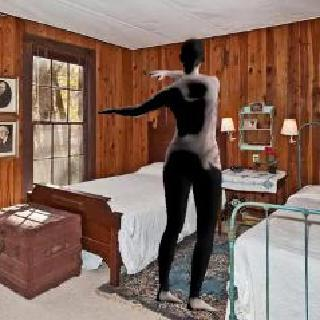
\includegraphics[scale=0.3]{80_15_c0002_85.jpg}
\end{subfigure}
\begin{subfigure}{.19\textwidth}
  \centering
  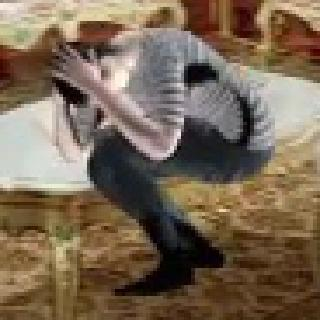
\includegraphics[scale=0.3]{ung_77_09_c0001_67.jpg}
\end{subfigure}
\begin{subfigure}{.19\textwidth}
  \centering
  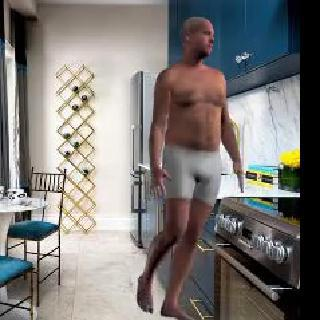
\includegraphics[scale=0.3]{ung_91_62_c0003_87.jpg}
\end{subfigure}
\begin{subfigure}{.19\textwidth}
  \centering
  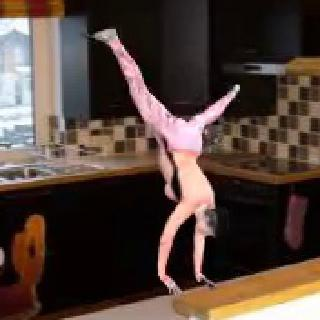
\includegraphics[scale=0.3]{ung_144_02_c0006_2.jpg}
\end{subfigure}\\
\begin{subfigure}{.2\textwidth}
\centering
  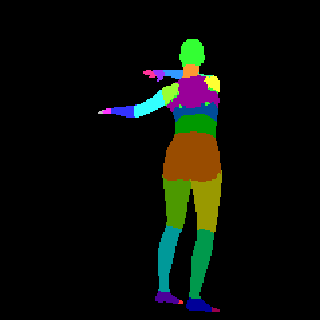
\includegraphics[scale=0.3]{80_15_c0002_segm_85.png}
\end{subfigure}%
\begin{subfigure}{.19\textwidth}
  \centering
  
\includegraphics[scale=0.3]{ung_77_09_c0001_segm_67.png}
\end{subfigure}
\begin{subfigure}{.19\textwidth}
  \centering
  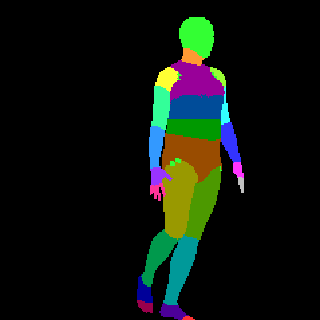
\includegraphics[scale=0.3]{ung_91_62_c0003_segm_87.png}
\end{subfigure}
\begin{subfigure}{.19\textwidth}
  \centering
  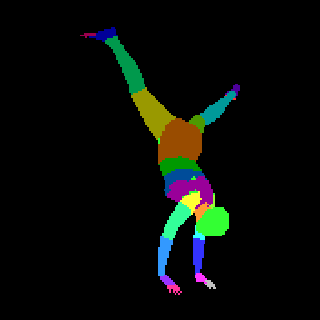
\includegraphics[scale=0.3]{ung_144_02_c0006_segm_2.png}
\end{subfigure}

\caption{First row: sample images. Second row: corresponding ground truths}
\label{dataset:samples}
\end{figure}

% Chapter 2

\chapter{Network study} % Main chapter title

\label{Chapter2} % For referencing the chapter elsewhere, use \ref{Chapter1} 

%----------------------------------------------------------------------------------------


%----------------------------------------------------------------------------------------

\section{General Segmentation Purposed Networks}

\subsection{Experimental Procedure}\label{method}

In this section the steps that will be followed when studying each network will be defined. The main purpose of doing so is to create a standardized procedure that helps in the reproduction of results, the study of the networks and the comparison between them. \newline

First, with several and short runs, the hyper-parameters of the code, such as learning rate, batch size, among others, are modified just to obtain the best combination and cope with other type of problems such as memory consumption. Once this has been done and the hyper parameters has been established the next step is to begin with ablation studies. However, and before that, is important to check if some more modifications have to be made in the code, such as including validation performance recording, if it does not have it, just to make sure proper results will be obtained.\newline

The ablation studies will consists on four modifications of the original network to see how it behaves. The modifications, that will be repeated for each network if possible, are:

\begin{itemize}
\item Doubling convolution filters
\item Data augmentation: mirroring and scaling
\item Class balancing through loss weighting
\end{itemize}

Before explaining each of the ablation procedures, it is convenient to explain the method that will be followed to apply them. First of all, the performance of the original network will be compared with the one with doubled filters. Then the best from the previous two regarding validation results will be compared to the network which includes data augmentation. Then, as before, the best from the previous comparison will be compared to the network with class balancing. Hence, the purpose of this ablation studies is, apart from seeing how the network behaves, to choose the best performing option. The training procedure is usually performed through 40k iterations (not epochs) on the training set, if another number is not specified. The performance result on the validation set is computed every certain  number of steps, usually 200, to avoid runs that are too time consuming. \newline

Finally, once the best performing network has been chosen it will be trained in a long run, always avoiding overfitting, and the network will be evaluated on the test set to obtain final results for this network. This results will, at the end, be useful to compare with the other networks studied.\newline

The first ablation or modification is to double the quantity of filters of each convolution layer of the network. The main purpose of this change is related to the relationship between the variability of the data and the complexity of the network. If the original network is not sufficiently complex (does not has enough parameters) to absorb the diversity of the data an increase in filters may help the structure to get  better results. However, if the original structure is already complex enough an increase in parameters will provoke, as usually, a reduction in the performance in the validation dataset due to the overfitting towards the training dataset. The purpose is then to study this possibilities.\newline

Regarding the next ablation study, data augmentation, the purpose is related to the first ablation procedure. To add more diversity to the data and to end up with a more robust network against variability, the data is augmented, mainly through mirroring and scaling. Mirroring in our case consists in a 180º degrees flip and scaling refers to the the image size modification. \newline

Finally, the third change is adding a weighting to the loss. This is due to the fact that in the selected dataset there is a clear problem of unbalanced classes(background occupies most of the pixels). Hence to compensate this, two strategies are devised to weight the loss regarding the weight of each class. As a multi class single label problem is faced (as it is semantic segmentation), the loss is computed through \textit{softmax crossentropy}. Hence and having this loss in mind, the weighting methods consist in:\newline

\textbf{Direct strategy}\newline

\begin{equation*}
L = -\sum_{i} y_{i}\log(softmax(x_{i}w_{i}))
\end{equation*}

where $y_{i}$ is the label or ground truth, $x_{i}$ is the output of the network and $w_{i}$ is the vector of weights. The index $i$ in this case refers to the class dimension in a one-hot encoding.\newline

\textbf{Outter strategy}\newline

\begin{equation*}
L = -\sum_{i}  w_{i}y_{i}\log(softmax(x_{i}))
\end{equation*}


In the first case, it can be seen that the weights are applied directly to the output values while in the second they are applied to the result of the crossentropy computation.\newline

Nevertheless, there  is one point left to state: how to choose the weights. Being C the total number of pixels in the training dataset, two methods have also been chosen in this case:\newline

\textbf{Inverse Frequency}\newline

\begin{equation*}
W_{i} = 1-\frac{C_{i}}{\sum_{i}C_{i}}
\end{equation*}

this weights will be marked as W1 throughout the work.\newline

\textbf{Exponential Weights}\newline

\begin{eqnarray*}
A = \frac{C}{max(C)}\\
B = \frac{1}{B}\\
W = B e^{-\frac{1}{4}\frac{B-mean(B)}{std{B}}} 
\end{eqnarray*}

in this case \textit{std} means standard deviation. This weights will be marked as W2 athrought the work.\newline

Hence, what has been stated will be the main methodological procedure for this study. Nevertheless, the implementation of the specific steps is subject to the progress of the job. That is, and as will be seen, modification of the methodological procedure or further implementations will be applied as needed and at the light of the results obtained in the previous sections. This is done with the purpose of not establishing a specific and fixed methodology but rather a base for a further, deep and dynamic development of the study. \newline

\subsection{ICNet: Image Cascade Network}

\subsubsection{Introduction}

Semantic segmentation methods based on CNN structures have improved largely the performance and have put offside methods based on hand crafted features. Among the CNN based methods there have been, mainly, two streams of development which have not been merged: high quality semantic segmentation methods and fast inference methods. In one hand, high quality methods, fueled initially by FCN (Fully Convolutional Networks), and further developed by works such as DeepLab or CRF (Conditional Random Fields), have centered their attention in obtaining as high as possible performance results. Thus, these methods have ended up without the possibility of being applied in real time scenarios. In the other hand, structures such as UNet or SegNet, have been created focused in high speed inference for semantic segmentation. Nevertheless and although these methods greatly raise the performance regarding efficiency, accuracy has been not maintained and has dropped to low levels. \newline

Hence, the main purpose of the design of the present network is to achieve fast semantic segmentation while maintaining decent prediction accuracy. Nevertheless, the problem is two sided: on one hand, low resolution images would reduce inference and running time but would yield coarse, blurry outputs. On the other, high resolution inputs would be unbearable for the objective just because they would increase substantially inference time. Thus, to accomplish the objective, low resolution images are used to high efficiency processing and to obtain a first but low quality segmentation feature map, while high quality is gained from high resolution images. Then, to merge both results a cascade framework is built in order to progressively refine segmentation predictions.

\subsubsection{Description}

The net is composed by three branches of different input resolutions and a cascade label guidance method (CCF: Cascade Feature Fusion Unit).\newline

\textbf{Low resolution}. The input is downsampled to 1/4 of the original resolution and is passed through a FCN-based PSPNet architecture, \parencite{Reference22}. The final output feature map, due to the pass through convolution layers, is 1/32 of the original resolution. After that the feature map is passed through several dilated convolution layers to enlarge the receptive field without downsampling the spatial size.\newline


\begin{figure}
\begin{center}
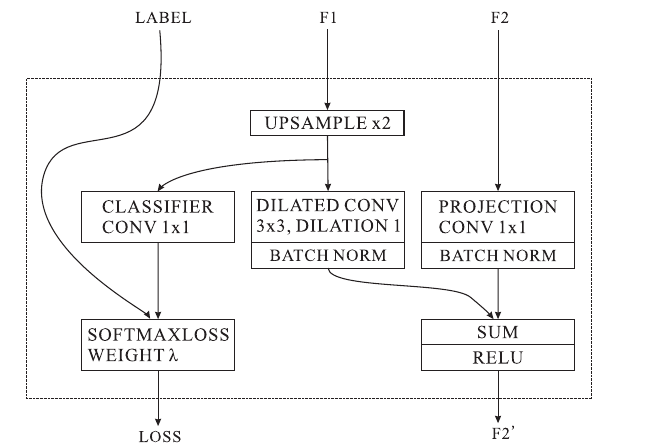
\includegraphics[scale=0.55]{ccf.png}
\caption{Cascade Feature Fusion unit. Two feature maps as inputs. One of the feature maps, F1, coming from a lower resolution branch, has half of the resolution than the other input.}
\label{ccf}
\end{center}
\end{figure}

\textbf{Middle resolution}. The input is reduced to a 1/2 of the original resolution and after going through the convolution layers the outputted feature map has a resolution of 1/16 of the original image. Then through the Cascade Feature Fusion unit this output is merged with the output of the low resolution branch by upsampling the latter by a factor of 2.\newline

\textbf{High Resolution}. As the middle resolution has already restored most semantic information the number of convolutions can be limited here. Three convolution layers are devised with kernel size 3x3 and stride 2 to go from an original resolution input to a 1/8 dowsample feature map. This feature map is combined through the CCF with the factor 2 upsampled map from the median resolution branch. Then the result is upsampled to resolution 1/4 and passed through a projection convolution.\newline

\textbf{CCF: Cascade Feature Fusion}. As seen two feature maps are had. One, which comes each time from the lower resolution branch to the respective branch, has half the resolution. Then a dilated convolution with kernel size 3x3 and dilation 1 is applied to refine upsampled features. Following batch normalization layers are applied to each feature map and then a element wise SUM followed by a \textit{ReLU} layer, ending up with both layers fused. This structure can be seen at Figure \ref{ccf}\newline

\begin{figure}
\begin{center}
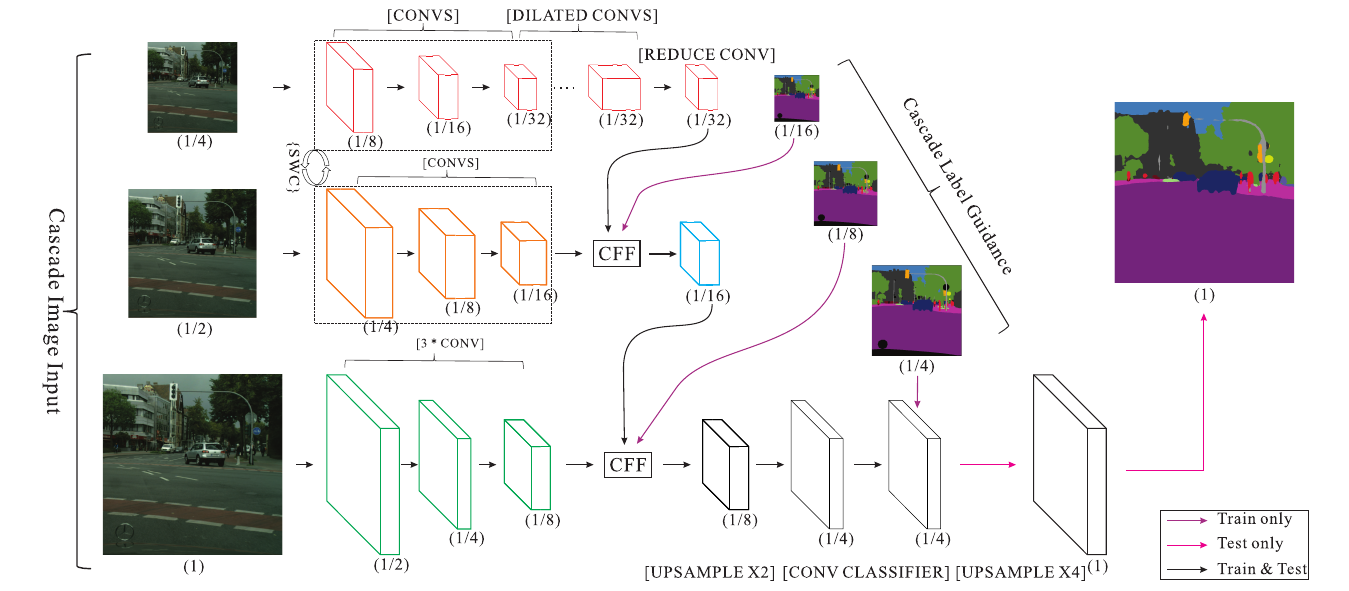
\includegraphics[scale=0.45]{icnet.png}
\caption{Sketch of the architecture of ICNet: the three resolution branches the CCFs and the points were the loss is computed. Also the specification of the use of each of the parts in terms of training and testing.}
\label{icnet}
\end{center}
\end{figure}

Finally and regarding training, a softmax crossentropy loss is added to each branch producing three losses $L_{1}$, $L_{2}$ and $L_{3}$,

\begin{equation*}
L = \lambda_{1}L_{1} + \lambda_{2}L_{2} + \lambda_{3}L_{3}
\end{equation*}

where the $\lambda_{i}$ are the weights applied to each branch loss. The network is then trained regarding the total loss. Has to be noted that, to gain efficiency at testing time,  the low resolution branches are not used and that the full resolution branch is expanded with one more upsampling to obtain an output of the resolution of the initial input. A global view of the architecture can be checked at Fig \ref{icnet}.

\subsubsection{Results}

The code used for this section can be found at \href{https://github.com/hellochick/ICNet-tensorflow}{hellochick/ICNet-Tensorflow}.\newline

\textbf{Code adaptation}. Several changes were made to the code in order to be able to apply it to our dataset and environment:

\begin{itemize}
\item Data input files.
\item Input Size
\item Number of classes and the ignored label.
\item Enable loading of pretrained model by avoiding the load of final classification
 layers.
\item Add validation structure
\begin{itemize}
\item Created another instance of the class \textit{Network}. 
\item Establish the parameters as non trainable. 
\item Copy the trained network into the validation network each time validation is carried out. 
\end{itemize}
\item Add metrics:  F1, precision, recall, accuracy and accuracy per class.
\item Add the possibility to weight loss according to each class importance.
\end{itemize}

After several finetunning purposed runs of the program the hyperparameters of the network has been set to the following values:

\begin{itemize}
\item Batch size 64
\item Learning rate 0.01 and poly learning rate with power 0.9
\item Momentum 0.9 and weight decay 0.0001
\end{itemize}

The optimizer used corresponds to a momentum optimizer.\newline

\textbf{Ablation Results}. To see which of the different possible configurations was the best performing one, several runs have been carried out regarding number of filters, data augmentation and class balancing. The number of steps for training have been defined as 40000, the last 20000 with batch normalization parameter updating.\\

First of all, the performance on the validation set  of normal structure and  of the same one but with filters doubled are compared.

\begin{table}[h!]
  \begin{center}
    
    \begin{tabular}{|c|c|c|c|} % <-- Changed to S here.
      \textbf{Architecture} & \textbf{mIoU ($\%$)} & \textbf{Accuracy ($\%$)} & \textbf{F1 ($\%$)} \\
      \hline
      Normal & 38.19 & 94.64 & 88.17\\
      \hline
      Doubled filters & 27.51 & 93.01 & 84.97\\  
      \hline
      Normal + Data Aug. & 32.60 & 91.15 & 91.61\\
    \end{tabular}
    \caption{Performance results on validation dataset for the normal structure and the architecture with doubled filters.}
    \label{icnet:table1}
  \end{center}
\end{table}

As seen in table \ref{icnet:table1}, doubling the filters has not produced any gains. In Figure \ref{icnet:filters} the behavior of the losses as well as the metric mIoU in both training and validation datasets can be observed.  It is seen that both developments are close to saturation, although in the doubled filters net there seems to be still space for training. Nevertheless, the evolution and results on the validation set are worse in this latter structure than in the normal one. Thus, and given this fact together with the saturation behavior, the normal net is preferred against the one with doubled filters.\newline

\begin{figure}
\centering
\begin{subfigure}{.5\textwidth}
  \centering
  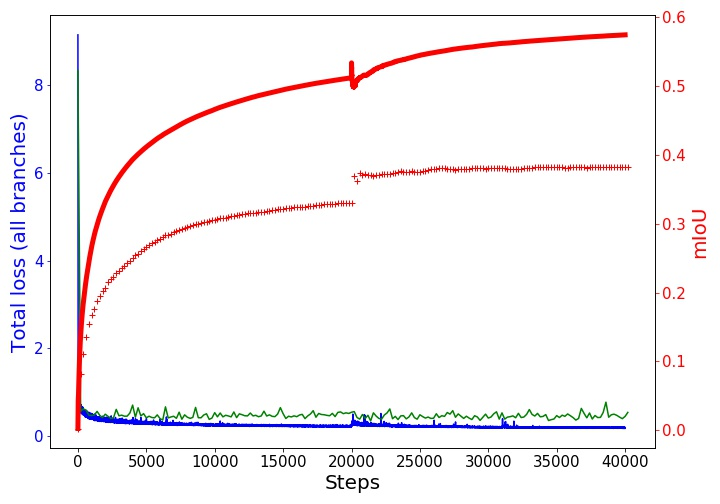
\includegraphics[width=.95\linewidth]{icnet_res_1.jpg}
\end{subfigure}%
\begin{subfigure}{.5\textwidth}
  \centering
  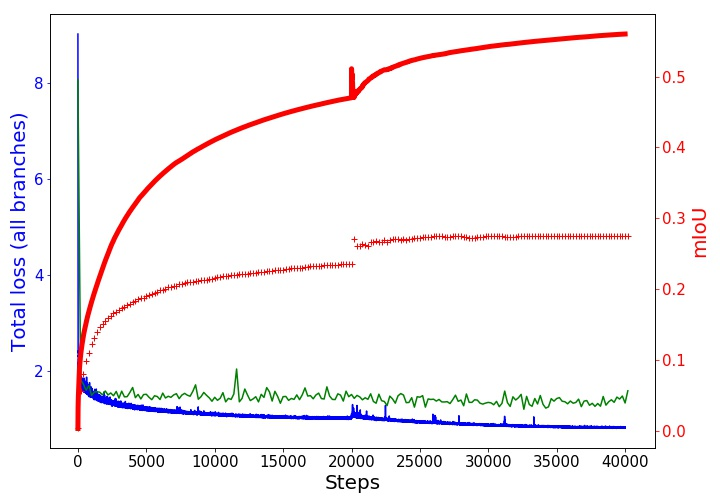
\includegraphics[width=.95\linewidth]{icnet_res_2.jpg}
\end{subfigure}
\caption{Loss plots for both normal (left) and with doubled filters (right) ICNet architectures. (Green) Validation loss, (Blue) Training Loss,  training mIoU (red solid line) and validation mIoU (red crosses). }
\label{icnet:filters}
\end{figure}

Hence, and according to the methodology established in Section \ref{method}, the results obtained next are the comparison between the best previous ablation, that is the structure without doubled filters, and the same net but with data augmentation. This is done with the intuition that the mirroring and scaling would help in making the net more robust during training and hence obtain a better result in the validation set. The results can be observed also in table \ref{icnet:table1}. Has to be noted that, although the results regarding mIoU, and also accuracy, are worse compared to not using data augmentation, the performance regarding F1 is better. Nevertheless, as our metric of preference is mIoU we still have the normal structure as the best performing one.\newline

Following, the normal structure is compared to the four different ways of applying class balancing to loss values (as established in \ref{method}). Now the comparison is done through mIoU but also through accuracy per class to see the effects of the loss weighting. The results can be observed in table \ref{icnet:table2}.\newline

\begin{table}[h!]
  \begin{center}
    \resizebox{\textwidth}{!}{
    \begin{tabular}{|c|c|c|c|c|c|c|c|c|c|c|c|c|c|c|c|c|c|c|c|c|c|} % <-- Changed to S here.
    &\textbf{mIoU ($\%$)}&\multicolumn{14}{c|}{\textbf{Accuracy per Class}($\%$)}\\
    \hline
      \textbf{Architecture} & \textbf{All Classes} & \textbf{All Classes}& \textbf{Background} & \textbf{Head} & \textbf{Torso} & \textbf{U.Legs}& \textbf{L.Legs} & \textbf{Neck} & \textbf{Shoulder} & \textbf{U.Arms}& \textbf{L.Arms}& \textbf{Feets}& \textbf{Hands}& \textbf{Fingers} & \textbf{Toes}  \\
      \hline
      Normal & [38.2] & 48.7 & 98.9 & 84.9 & 74.78 & 64.3 & 53.8 & 64.0 & 54.2 & 52.7 & 39.5 & 32.3 & 19.8 & 9.3 & 9.5 \\
 	  \hline
      W1 (Outer) & 37.5 & 52.3 & 97.7 & 90.0  & 74.8 & 70.9 & 61.7 & 60.9 & 56.0 & 57.34 & 50.1 & 38.9 & 22.9 & 10.2 &  11.3\\  
      \hline
      W1 (Direct) & 6.5 & 7.9& 99.9 & 6.13 & 15.5 & 7.7 & 0.8 & 0.0  & 4.7 & 1.9 & 0.0 &3.6 & 0.0 & 0.0 & 0.0\\
      \hline
      W2 (Outer) & 25.8 & [54.8] & 89.2 & 89.3 & 61.6 & 64.1 & 65.2 & 72.4 & 60.3 & 47.0 & 46.03 & 52.35 & 33.4& 31.0 & 36.9 \\
      \hline
      W2 (Direct) & 25.5 & 34.0 & 99.3 & 78.7 & 70.7 & 70.0 & 59.0 & 1.9 & 8.9 & 32.9 & 15.7 & 7.1 & 0.5 & 0.0 & 0 .0 \\
    \end{tabular}}
    \caption{Performance results on validation dataset for the normal structure and the architecture with loss weighting for each setup. Here W1 indicates the inverse frequency weithing and W2 the exponential weighting. Best values enclosed in [].}
    \label{icnet:table2}
  \end{center}
\end{table}

Although the  result of the loss weighting using the outer approach and the first set of weights has a performance similar to the normal structure, none of the results has surpassed the performance of the original structure. It can be observed, nonetheless, that the direct weighting is the worse in terms both of per class accuracy and mIoU. Although the first setup, among the weighting methods, has acquired the best mIoU result, the best balancing between classes in terms of accuracy has been achieved by the same method, that is outter balancing, but with the second set of weights.\newline


\textbf{Final Results}. With the best setup regarding validation results, in this case the normal one with no additions, a training of 90k iterations is performed to achieve the best possible results.\newline

\begin{table}[h!]
  \begin{center}
    
    \begin{tabular}{|c|c|c|c|} % <-- Changed to S here.
      \textbf{Architecture} & \textbf{mIoU ($\%$)} & \textbf{Accuracy ($\%$)} & \textbf{F1 ($\%$)} \\
      \hline
      Normal & 45.14 & 95.76 & 89.73\\
    \end{tabular}
    \caption{Performance results on test set for the normal structure with a training of 90k.}
    \label{icnet:table3}
  \end{center}
\end{table}

In table \ref{icnet:table3} the results regarding mIoU, accuracy and F1 score for the normal structure in the test set and for 90k steps of training are presented. As it is obvious the performance is higher but not as much as expected taking into account that training steps more than doubled.\newline

\begin{figure}
\centering
\begin{subfigure}{.19\textwidth}
\centering
  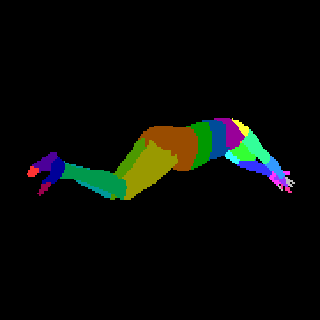
\includegraphics[scale=0.3]{ung_126_09_c0008_segm_85_gt.png}
\end{subfigure}
\begin{subfigure}{.19\textwidth}
  \centering
  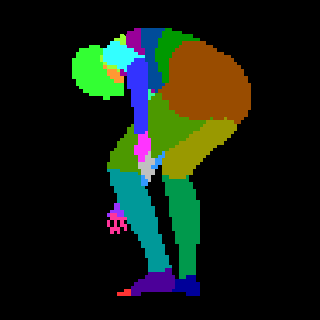
\includegraphics[scale=0.3]{ung_137_31_c0008_segm_77_gt.png}
\end{subfigure}
\begin{subfigure}{.19\textwidth}
  \centering
  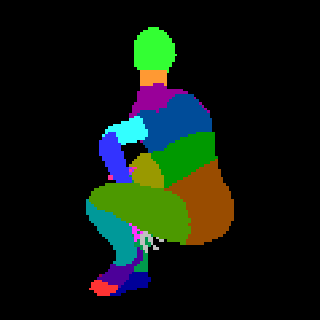
\includegraphics[scale=0.3]{19_12_c0006_segm_29_gt.png}
\end{subfigure}
\begin{subfigure}{.19\textwidth}
  \centering
  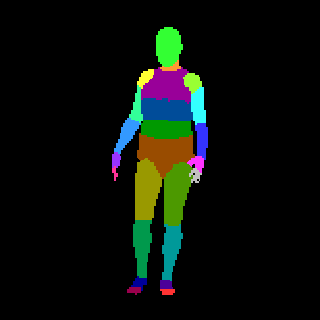
\includegraphics[scale=0.3]{ung_144_34_c0008_segm_39_gt.png}
\end{subfigure}\\
\begin{subfigure}{.2\textwidth}
\centering
  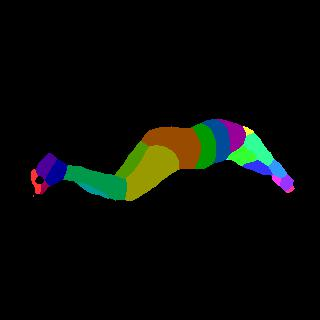
\includegraphics[scale=0.3]{ung_126_09_c0008_85.jpg}
\end{subfigure}%
\begin{subfigure}{.19\textwidth}
  \centering
  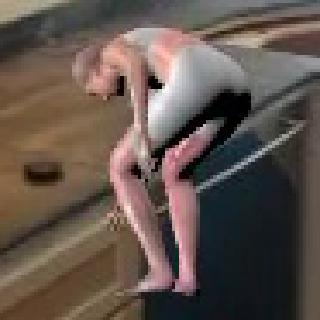
\includegraphics[scale=0.3]{ung_137_31_c0008_77.jpg}
\end{subfigure}
\begin{subfigure}{.19\textwidth}
  \centering
  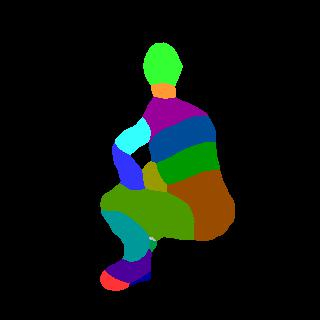
\includegraphics[scale=0.3]{19_12_c0006_29.jpg}
\end{subfigure}
\begin{subfigure}{.19\textwidth}
  \centering
  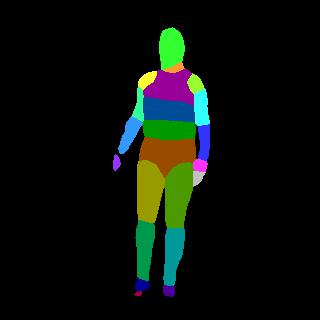
\includegraphics[scale=0.3]{ung_144_34_c0008_39.jpg}
\end{subfigure}

\caption{First row: ground truth examples. Second row: inference results with best ICNet model}
\label{icnet:inference}
\end{figure}



In Figure \ref{icnet:inference} qualitative results can be observed regarding the original structure with the 90k training.

\subsubsection{Analysis and Conclusions}

Regarding results shown in table \ref{icnet:table1}, we can see that the normal net has got a better result in the validation set than the net with filters doubled. When the filters of a net are doubled, the parameters of the net, logically, get doubled. This can lead to two ends: the first, if the data is sufficiently complex to allow the net to train without overfitting, the results get better due to capturing more patterns and information, or, the second, that the excess filters make the whole net overfit to the training data since they capture elements only present in the training data but not in the validation. Hence, by the results shown, it is clear that what happened corresponds to the second case. This can also be seen in Figure \ref{icnet:filters} where the validation results are much worse almost at every step during the training for the doubled filters net. This clearly indicates, comparatively, an overfitting problem of the net.\newline

Regarding the case of data augmentation, also in table \ref{icnet:table1}, the problem may reside in that spatial information is important for learning the characteristics of the data. Hence, the distortions/modifications caused by the data augmentation, maybe disrupt the structure of this spatial informations. The main intention of data augmentation is make the net more robust to changes in the data, but maybe this effect is overcame by the disruption on the spatial data information.\newline

In the case of the loss weighting scheme several statements can be made. First of all, the direct application of the weights has no use since it has not balanced the results at all. Next, regarding the outer application, although with the exponential weights the classes are more balanced in terms of accuracy (even the upper legs have obtained a better accuracy per class result than background), the result regarding mIoU is lower than in the original network. Comparing the results between the two outer method instances, one with the inverse frequency weights and the other with the exponential weights, one important thing can be commented: exponential weights seem to balance classes better while inverse frequency weights do not but obtain a better mIoU result. This can be due to the fact that trying to balance perfectly classes that account for a little area produces a poorer results if the main performance metric is related to area comparison.\newline

One important point to comment is the jump in the performance metric that appears in Figure \ref{icnet:filters}. This jump corresponds to the inclusion of batch normalization variables into the trainable variables. Batch normalization consists in the following formulation\newline

\begin{equation}
\beta +\frac{\gamma(x-\mu)}{\sigma}
\end{equation}

In the first part of the training these variables, $\beta$,$\gamma$,$\mu$ and $\sigma$ are not trained and correspond to fixed random values. When they are included into training its value gets adapted to the dataset. It is important then its inclusion. Nevertheless, the point at which they are included it is not significant since the behavior of the performance ens up being the same. Thus, it is only important that these inclusion into trainable variables takes place to obtain a proper training.\newline 

Regarding the final results on the test set, what can be established is that the structure is near saturation. That is training it more will not improve substantially the results. This can be deduced from Figure \ref{icnet:filters}, where already was showing a little saturation, and from the fact that, with even more than doubling the steps, the results have not improved much. Also important to comment is the fact that, compared to the performance of the network used in the original paper on the Cityscapes dataset \parencite{Reference23} the result regarding mIoU is quite poor, since the authors obtain 67.7$\%$ mIoU on the test set. Nevertheless, in the case of the Cityscapes dataset the number of classes is 19.\newline

On of the main reasons for this drop in performance could be that in our dataset a large (regarding pixel appearance frequency) and varied background which implies that the network spends part of its training learning to identify the background.\newline

Nevertheless, if a look is taken at the qualitative results in Figure \ref{icnet:inference}, it can be seen that they are quite acceptable. This statement is regarding body part definition and overall appreciation of the  constituents of the body. The only body parts that lack of substantial definition are the extremities, such as fingers and toes which are bad defined or even not identified. Regarding variety of positions and occlusions of  body parts it can be observed that the results are positive since the network has managed to learn the variety of body poses and occlusions regarding the body going out the frame.\newline

As a conclusion, the results have been positive but not as high as expected. Also and surprisingly, all the ablation studies have resulted in no improvement of the performance results. In the case of the class balancing scheme, the direct method has proven to be a bad choice, hence it is discarded for further networks to be studied.\newline

\subsection{SegNet}

\subsubsection{Introduction}

Regarding our task, which is semantic pixel-wise segmentation, most recent deep architectures share common or similar encoding parts, such as VGG-16 or ResNet. Even so, some of those approaches adapt structures oriented to one specific tasks, such as classification, to other tasks, such as semantic segmentation. This two facts have two big implications in the resulting networks. First, and commonly, the number of trainable parameters of the structure ascends to orders of hundreds of millions which makes difficult end-to-end training. This opens the way to multistage strategies such as task decoupling, appending heads to pre-trained base networks and other methods to ease the training process. Secondly, usually the output lacks of required definition, that is, appears coarse. This is mainly due to the reduction of resolution in the feature maps produced by max-pooling layers and other sub-sampling procedures. Solving these two hurdles will enable and efficient training and inference in terms of both memory and computation time. \newline

Thus, the design and development of Segnet has been focused on both problems. This means having the requirement of a high quality mapping between low resolution features and  input resolution pixel classification but without deepening or loading too much, just to avoid difficulties and inefficiencies at both inference and training time. 

\subsubsection{Description}

\begin{figure}[!htbp]
\begin{center}
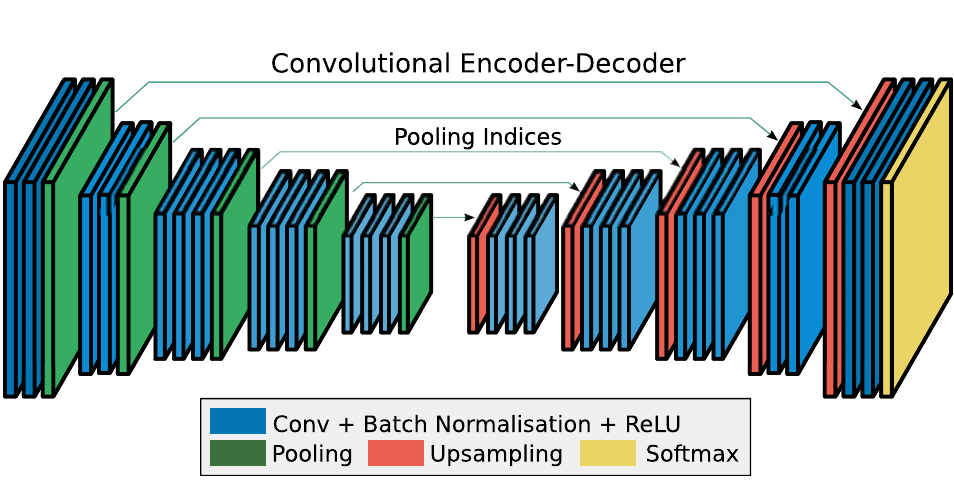
\includegraphics[scale=0.45]{seg_net.png}
\caption{Sketch of the architecture of SegNet: the encoder, the decoder and the final classification layer, as well as the skip connections between encoder and decoder.}
\label{segnet}
\end{center}
\end{figure}

Segnet consists of three components: encoder, decoder and a final classification layer. The encoder is composed by the 13 convolution layers of VGG-16, from which the final fully connected layers have been subtracted reducing then the number of parameters. Each encoder layer has a relative decoder layer and hence 13 decoding layers are had, followed by a multi-class softmax classifier. A representation of the SegNet structure can be observed at Figure \ref{segnet}.\newline

The \textit{encoder} part is composed as a stack of the following structure: convolution layer with ReLU activation, batch normalization and max-pooling layer of window 2x2 with stride 2. This last layer helps the net to be more robust against shifts and space variations, however several layers of pooling can induce loss of spatial resolution. Hence, to avoid this loss the indexes of the max-pooling layers are stored to be used once again at the decoder part. \newline

\begin{figure}[!htbp]
\begin{center}
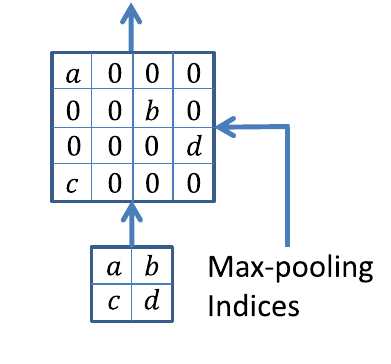
\includegraphics[scale=0.5]{seg_idx.png}
\caption{Illustration of the use of the saved max-pooling indexes during the upsampling procedure.}
\label{segidx}
\end{center}
\end{figure}

Then the \textit{decoder} part upsamples the received feature maps using the stored pooling indexes as depicted in \ref{segidx}, thus avoiding any learning parameter in the upsampling step. As the resulting output is notably sparse, a convolution layer and batch normalization layers are applied to obtain better resolution and denser outputs. Has to be noted that only storing the pooling indexes is computationally more efficient than storing all encoder feature maps, and regarding pragmatic use, there is only a little loss on resolution.\newline 

And finally the last component is the classification layer with a softmax classifier giving K channel probabilities (one for each class). The class selected is the one with maximum probability.\newline

Among the variants appearing in the original paper, SegNet basic has been chosen for study. It consist of a smaller version of Segnet which only has four encoders and four decoders. The main differences, apart from size, are that no bias and ReLu units are used in the decoder part and that a constant kernel size of 7 x 7 is used in all encoder and decoder layers.\newline

\subsubsection{Results}

The code used for this section can be found at \href{https://github.com/tkuanlun350/Tensorflow-SegNet}{tkuanlun350/Tensorflow-Segnet}.\newline

\textbf{Code adaptation}. Several changes were made to the code in order to be able to apply it to our dataset and environment:

\begin{itemize}
\item Image size defintion
\item Number of classes
\item Form of access to dataset
\item Program parameters for ablation purposes.
\item Add metrics:  F1, precision, recall, accuracy and accuracy per class.
\item Possibility of doubling the filters at each convolution layer.
\item Added data augmentation methods: mirroring and scaling.
\end{itemize}

After several finetunning purposed runs of the program the hyperparameters of the network has been set to the following values:

\begin{itemize}
\item Batch size 32 (16 if memory problems)
\item Learning rate 0.01
\end{itemize}

As optimizer Adam is used.\newline

\textbf{Ablation Results}. To see which of the different possible configurations was the best performing one several runs have been carried out regarding number of filters, data augmentation and class balancing. The number of steps for training have been defined as 40000.\newline

As first results obtained,  the performance in the validation set for the original structure and for the structure with doubled filters are had. Results can be found in table \ref{segnet:table1}. As can be seen the doubled filters structure obtains a better result regarding all the performance metrics than the original structure. Hence, and following the procedure established in methodology, this modification is set as the momentarily best structure and the following ablations will be added to it.\newline

\begin{table}[h!]
  \begin{center}
    
    \begin{tabular}{|c|c|c|c|} % <-- Changed to S here.
      \textbf{Architecture} & \textbf{mIoU ($\%$)} & \textbf{Accuracy ($\%$)} & \textbf{F1 ($\%$)} \\
      \hline
      Normal & 38.80 & 94.87 & 54.34\\
      \hline
      Doubled filters & 39.17 & 94.79  & 54.49 \\  
      \hline
      Doubled Filters + Data Aug. & 23.28 & 89.24 & 33.21\\
    \end{tabular}
    \caption{Performance results on validation dataset for the original structure and the architecture with doubled filters. Also performance metrics included for the best of the two previous modifications plus data augmentation.}
    \label{segnet:table1}
  \end{center}
\end{table}

Regarding the case of data augmentation the results can also be observed at table \ref{segnet:table1}. In this case, as with ICNet, the results has not improved with the two methods of data augmentation but the contrary, it has got poorer. In any of the performance metrics the result is better for the case with data augmentation. In Figure \ref{segnet:filters}, the representation of training for both the doubled filter structure and the same but with data augmentation can be observed. As seen in the images, in the data augmentation case there is less distance between the performance in the training set and in the validation set than in the case without data augmentation. Nevertheless, the performance is worse in the data augmentation case where it does not grow at the same pace than in the case without it.\newline

\begin{figure}
\centering
\begin{subfigure}{.5\textwidth}
  \centering
  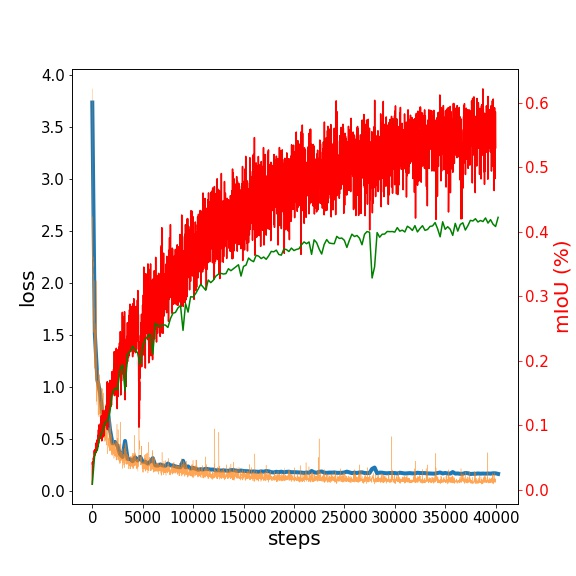
\includegraphics[width=.95\linewidth]{seg_res_1.jpg}
\end{subfigure}%
\begin{subfigure}{.5\textwidth}
  \centering
  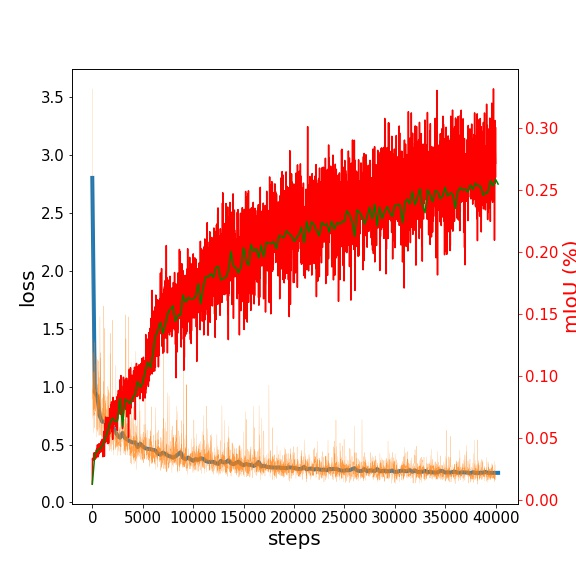
\includegraphics[width=.95\linewidth]{seg_res_2.jpg}
\end{subfigure}
\caption{Loss plots for both doubled filters (left) and doubled filters with data augmentation (right) Segnet architectures. (Blue) Validation loss, (Orange) Training Loss,  training mIoU (red solid line) and validation mIoU (green line). }
\label{segnet:filters}
\end{figure}

Next results, as shown in table \ref{segnet:table2}, are in regard the weighting scheme strategy. In this case, the direct strategy has been ruled out due to its results with the ICNet network. Hence, only has been taken into account the outer strategy. In the table the performance regarding global mIoU and Accuracy per class is considered among the doubled filters structure and its weight balancing variants. As seen, the best performing one, regarding mIoU, turns out to be the doubled filter structure without any balancing scheme. Nevertheless, if overall accuracy is taken into account, the best performing network is the doubled filter structure plus outer weighting scheme with exponential weighting.\\

\begin{table}[h!]
  \begin{center}
    \resizebox{\textwidth}{!}{
    \begin{tabular}{|c|c|c|c|c|c|c|c|c|c|c|c|c|c|c|c|c|c|c|c|c|c|c|} % <-- Changed to S here.
    &\textbf{mIoU ($\%$)}&\multicolumn{12}{c}{\textbf{Accuracy per Class}($\%$)}\\
    \hline
      \textbf{Architecture} & \textbf{All Classes} & \textbf{All classes}&\textbf{Background} & \textbf{Head} & \textbf{Torso} & \textbf{U.Legs}& \textbf{L.Legs} & \textbf{Neck} & \textbf{Shoulder} & \textbf{U.Arms}& \textbf{L.Arms}& \textbf{Feets}& \textbf{Hands}& \textbf{Fingers} & \textbf{Toes}  \\
      \hline
      Double Filters & [39.17]  & 49.9 & 99.1 & 84.2 & 70.9 & 63.2 & 58.4 & 58.1 & 51.8 & 52.7 & 43.9 & 39.9 & 28.8 & 12.4 & 9.8 \\
 	  \hline
      DF + W1 (Outer) & 38.8 & 55.6 & 97.5 & 90.3 & 74.2 & 66.8 & 61.8 & 58.3 & 65.1 & 62.0 & 49.6 & 42.0 & 36.3 & 25.3 &  14.2\\  
      \hline
      DF + W2 (Outer) & 21.65 & [56.3] & 78.18 & 79.8 & 65.6 & 60.0 & 57.1 & 85.8 & 71.1 & 52.5 & 51.8 & 44.2 & 41.7 & 34.1 & 38.4 \\

    \end{tabular}}
    \caption{Performance results on validation dataset for the doubled filter structure and the same architecture but with loss weighting for each setup. Here W1 indicates the inverse frequency weithing and W2 the exponential weighting (DF, i.e. doubled filters). Between brackets the best perfoming scheme in both mIoU and mean Accuracy per class.}
    \label{segnet:table2}
  \end{center}
\end{table}


\textbf{Final Results}. \newline

As the best model regarding mIoU has been the one with the filters doubled, a run of 90k steps has been carried out. The results on the test set can be seen at table \ref{segnet:table3}. As seen the performance on test results has dropped a bit compared to validation results on table \ref{segnet:table1}. Also to remark is the fact that the performance regarding the mteric F1 is also quite low.\newline


\begin{table}[h!]
  \begin{center}
    
    \begin{tabular}{|c|c|c|c|} % <-- Changed to S here.
      \textbf{Architecture} & \textbf{mIoU ($\%$)} & \textbf{Accuracy ($\%$)} & \textbf{F1 ($\%$)} \\
      \hline
      Normal & 33.59 & 94.62 & 44.32\\
    \end{tabular}
    \caption{Performance results on test set for the doubled filters structure with a training of 90k.}
    \label{segnet:table3}
  \end{center}
\end{table}

In figure \ref{segnet:inference} examples of the inference produced by the doubled filters Segnet structure can be observed. Note the lack of definition in most of the cases and how several parts are confused (for example, toes; in general those who have a left-right version).\newline

\begin{figure}
\centering
\begin{subfigure}{.19\textwidth}
\centering
  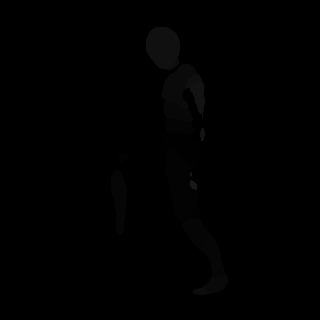
\includegraphics[scale=0.3]{36_04_c0001_segm_30.png}
\end{subfigure}
\begin{subfigure}{.19\textwidth}
  \centering
  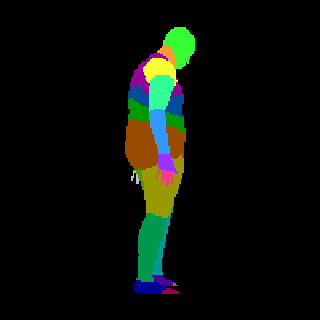
\includegraphics[scale=0.3]{36_16_c0002_segm_34.png}
\end{subfigure}
\begin{subfigure}{.19\textwidth}
  \centering
  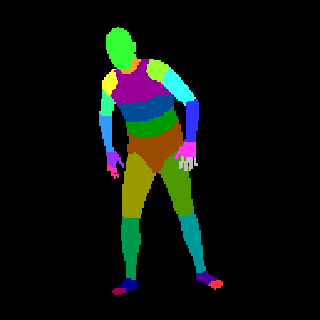
\includegraphics[scale=0.3]{104_52_c0002_segm_38.png}
\end{subfigure}
\begin{subfigure}{.19\textwidth}
  \centering
  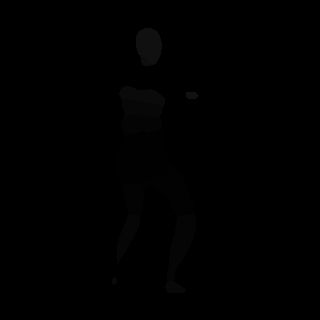
\includegraphics[scale=0.3]{ung_133_25_c0001_segm_29.png}\\
\end{subfigure}\\
\begin{subfigure}{.198\textwidth}
\centering
  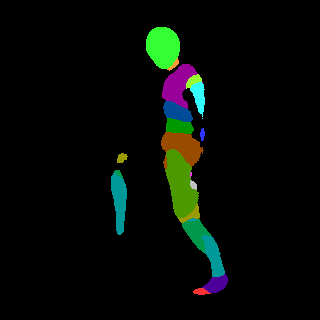
\includegraphics[scale=0.295]{36_04_c0001_segm_30_seg.png}
\end{subfigure}%
\begin{subfigure}{.19\textwidth}
  \centering
  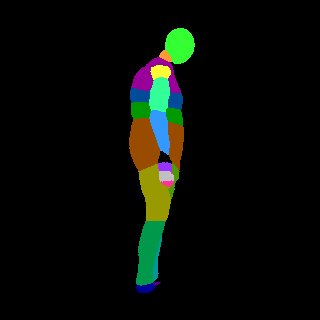
\includegraphics[scale=0.295]{36_16_c0002_segm_34_seg.png}
\end{subfigure}
\begin{subfigure}{.19\textwidth}
  \centering
  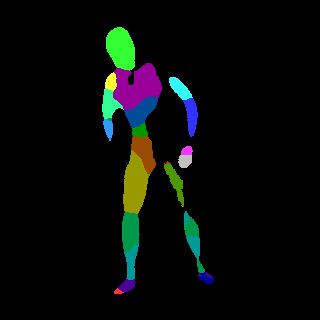
\includegraphics[scale=0.295]{104_52_c0002_segm_38_seg.png}
\end{subfigure}
\begin{subfigure}{.189\textwidth}
  \centering
  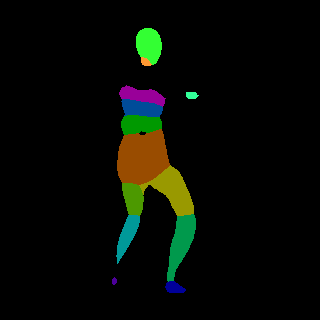
\includegraphics[scale=0.296]{ung_133_25_c0001_segm_29_seg.png}
\end{subfigure}

\caption{First row: ground truth examples. Second row: inference results with best Segnet model.}
\label{segnet:inference}
\end{figure}

\subsubsection{Analysis and Conclusions}

Regarding results shown in table \ref{segnet:table1}, it can be seen that the doubled filter structure has a better performance in the validation set. This can indicate that, denoted the variability in the data and the complexity of the original structure, an augmentation of the complexity of the structure, in our case by doubling the convolution filters, improves its result because it is able to capture more patterns and structures in the data. If the complexity of the original structure were enough the effect of doubling the filters would be a loss in the performance in the validation dataset. In our case, due to the size of SegNet (only 8 stacks in total), it was logical that it would be benefited from the increase in complexity.\newline

Then, also looking at table \ref{segnet:table1}, it can be observed that the data augmentation addition has been of no profit for the performance of the structure. It could be that the data augmentation methods, mirroring and scaling, were not the best ones for this dataset. Adding other data augmentation procedures, such as noise addition, would help to clarify this idea. Nevertheless, although the performance is worse in the data augmentation case, it can be observed a phenomena that would be expected in a training to which data augmentation has been added. That is, the distance between the performance in the training set and in the validation set is less than in the case without data augmentation. This is due to the fact that while training the net gets more robust to variations in the inputs and hence is more prepared against unseen data, thus not downgrading so much its performance in the validation dataset. This phenomena can be observed at Figure \ref{segnet:filters}.\newline

Regarding the weighting scheme procedure (results shown in table \ref{segnet:table2}), the best performing structure, regarding mIou, is the one with no weighting scheme. However, regarding mean Accuracy per class, the best performing one is the doubled filter structure but with outer balancing and exponential weighting. This difference in the best performing network regarding the metric used has an explanation. As mIoU considers areas and its extension, it is highly influenced by the classes that occupy a large portion of the image. Hence, when classes are balanced the loss of definition in the high portion classes in favor of minority classes makes the mIoU performance drop down. Meanwhile, the accuracy as is a relative value that only considers the pixels inside the class it is not affected by the portion of the area to respect the whole image. This is the reason why the class balancing scheme helps to improve the mean accuracy per class but drops down the mIoU. Nevertheless, as our main metric is mIoU, our best structure is the doubled filters with no weighting scheme.\newline

In the case of the final results a great drop in the performance regarding mIoU has been observed in the test set compared with the validation results. It could be thought that overfitting during training was the cause of this, but the training and validation loss plot, as seen in Figure \ref{segnet:over} does not indicates clearly a case of overfitting. The results regarding mIoU are way down the published results on the SUN RGB-D dataset for the Segnet basic variant which is the one that we use. The published results withstand a value of 46.3 $\%$ mIoU. It also surprises the result regarding F1 metric which is quite low. This poor results can be observed in the qualitative results in Figure \ref{segnet:inference}, which show the lack of definition and lack of some body parts, as well as the confusion between some parts (those which have right-left counterparts).\newline

\begin{figure}
\centering
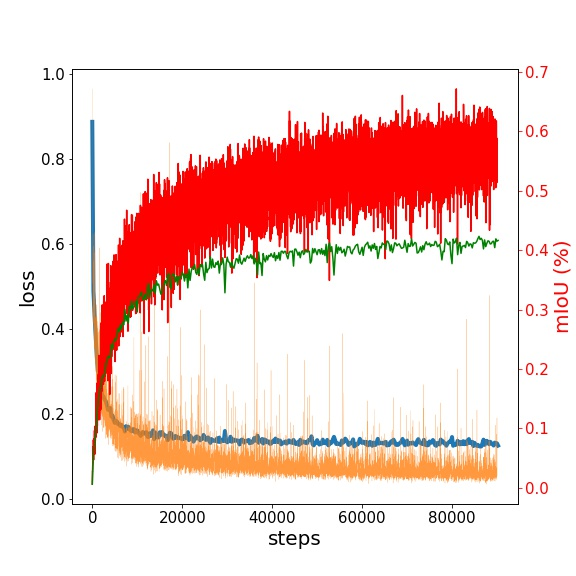
\includegraphics[scale=0.4]{seg_res_3.jpg}
\caption{Plot of the training for the doubled filters structure (90k steps). The values shown are training mIoU (red), validation mIoU (green), training loss (orange) and validation loss (blue). As seen no overfitting is apparent.}
\label{segnet:over}
\end{figure}

As a conclusion, in the Segnet basic case, the doubled filter structure have proved to be better than the original one, meaning that there was room for more complexity in the model given the variability/diversity of the data. Both data augmentation and balancing scheme has proven to be not useful in terms of mIoU. The final results, both qualitative and quantitative, out stand due to its low performance and quality.\newline
 
 
\newpage
\section{Specialized Networks}\label{specificstudy}


\subsection{Stacked Hourglass}

\subsubsection{Introduction}

Determining an accurate representation of the pose of a human body through its joints locations is useful for high level tasks such as action recognition. Early works devoted to pose determination used hand-crafted image features and elaborated structure prediction methods. However, with the advent of convolutional networks, the traditional pipeline was superseded and substituted by this new structure which provided significant improvements on the previously obtained results.\\

Following these new advances, the stacked hourglass model was developed specifically thought to the task of human pose estimation. As many convolutional procedures which produce pixel-wise outputs, the hourglass module captures features across different scales by the use of pooling and subsequent upsampling. Then multiple hourglass modules are stacked consecutively creating the final stacked hourglass network. This repetition allows for repeated top-down and bottom-up inference across different scales which, altogether with the intermediate supervision at the end of each module, enable a substantial improvement of performance.\\

In our case, and although the network was thought for pose estimation, the input and output of the network have been changed. This change obeys the need stemming from our semantic segmentation task. Nevertheless, with the exception of the input, output and loss function, the structure of the network has been kept the same proving its efficiency and versatility. Altogether with these changes, the two experiments described in the next sections have been carried out to try to state ways by which better results could be obtained either transforming the supervision pipeline or expanding the stacked hourglass network.\\

\subsubsection{Description}

\begin{figure}
\centering
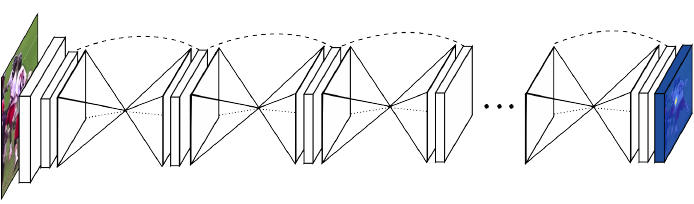
\includegraphics[scale=0.7]{stacked.png}
\caption{Simple representation of stacked hourglass network.}
\label{hourglass:stacked}
\end{figure}


The stacked hourglass network, as its own name indicates, is composed by several hourglass modules added in a consecutive manner. An overall example of the structure can be observed at Figure \ref{hourglass:stacked}. Each of the hourglass modules allow for bottom-up, top-down inference.\\

\begin{figure}
\centering
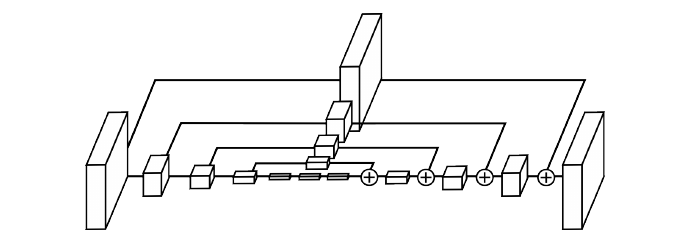
\includegraphics[scale=0.7]{hourmodule.png}
\caption{Representation of an hourglass module where each of the boxes represent a residual module.}
\label{hourglass:module}
\end{figure}

A hourglass module, as depicted in Figure \ref{hourglass:module}, is set up in the following way: convolutional and max pooling layers are used to capture features down to a certain resolution. Before each pooling, the network branches off an applies more convolutions to this branching. Once arrived at the lowest resolution, the upsampling process begins, in which nearest neighbor upsampling is used. During this process feature maps coming from the down sampling part and this up sampling part are merged by element wise addition. After reaching the input resolution two rounds of convolutions are applied to the output to obtain the final network prediction. In the original case probability heatmaps of the joint locations were generated, in our case, semantic segmentation of each of the body parts is produced as final output.\\

Due to performance improvements the convolution layers do not hold big filters: specifically, there are no filters bigger than 3x3. Also, reduction steps of convolution with filters 1x1 after each module, as well as residual modules, are implemented for the same reasons. A representation of a residual module can be observed at Figure \ref{hourglass:residual}.\\

\begin{figure}
\centering
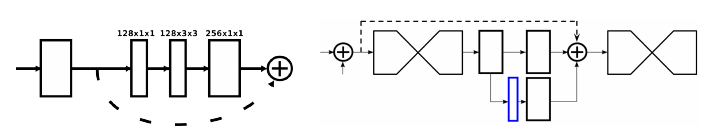
\includegraphics[scale=0.7]{residual.png}
\caption{\textbf{Left}: residual module used all through the network. \textbf{Right}: illustration of the intermediate supervision process. The  networks branches and a loss is applied to a semantic segmentation output. Then, this output, after having applied convolutions to match the number of channels is added to the main data pipeline. }
\label{hourglass:residual}
\end{figure}

It must be noted that, in the original network, the input was 256x256 while in our case is 320x320. Also, in the original network, the dimensions were reduced to 64 by a round of convolution with kernels 7x7 and stride 2, a residual module and a max pooling layer. In our case the max pooling layer has been deleted and the stride has been reduced to 1 in order to operate at the input resolution.\\

The fact of stacking several modules, where the input of the following is the output of the previous, provides a mechanism of repeated bottom-up, top-down inference, producing a continuous refinement of the estimates and features all over the image. The key to this point is the use of intermediate predictions at each module to which a loss applied. As a high level understanding of features is required to produce predictions the intermediate supervision is executed at the end of the upsampling process. This predictions came from a branch of the original pipeline and are reintroduced in the stream trough a 1x1 convolution to recover the required number of channels. This final output is served as input for the next module. A representation of these intermediate outputs can be found at Figure \ref{hourglass:residual}. Nevertheless, it must be noted that the las output of the network is the one used as final prediction, the intermediates are only used for training the network through a loss.\\

\subsubsection{Experimental Procedure}

In this section, a specialized networks will be tested with the SURREAL dataset: Stacked Hourglass. As the network was originally devoted to pose estimation some parts of the code has been changed. The most important ones are: data input and output streams and data reading, the loss and performance metrics. Regarding the loss it has been changed from \textit{sigmoid crossentropy loss with logits} to \textit{sparse softmax crossentropy with logits}, just to adapt it to the nature of the data. The metric was originally a measure of the distance error between the predicted body joint and the real one. This has been changed to the previously used metrics: mIoU, F1, accuracy and accuracy per class.\\

Also, regarding the last section of general networks, the experimental procedure is changed. Instead of applying variations such as data augmentation or loss weighting, the data structure and the network will be modified directly. Firstly, the plain network will be trained and tested with no modifications to see which are the baseline results to which compare with. Next, two experiments will be carried out to see if the performance results can be improved.\\

\begin{figure}
\centering
\begin{subfigure}{.19\textwidth}
\centering
  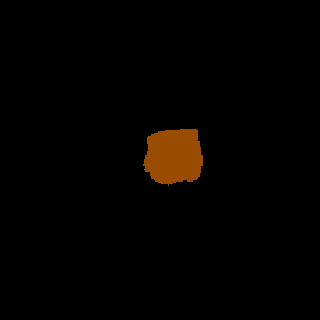
\includegraphics[scale=0.3]{02_05_c0005_segm_80_2c.png}
\end{subfigure}
\begin{subfigure}{.19\textwidth}
  \centering
  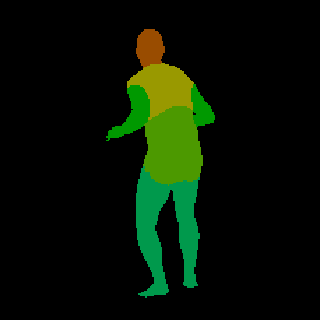
\includegraphics[scale=0.3]{02_05_c0005_segm_80_6c.png}
\end{subfigure}
\begin{subfigure}{.19\textwidth}
  \centering
  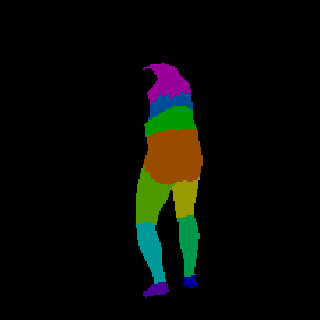
\includegraphics[scale=0.3]{02_05_c0005_segm_80_12c.png}
\end{subfigure}
\begin{subfigure}{.19\textwidth}
  \centering
  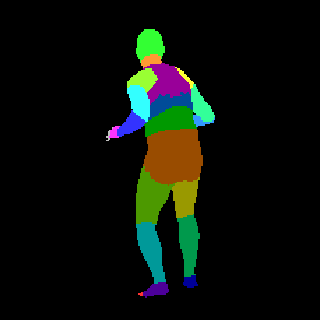
\includegraphics[scale=0.3]{02_05_c0005_segm_80_25c.png}\\
\end{subfigure}\\
\caption{Different ground truth resolutions, one for each module. The idea is to learn a progressive refinement of the real ground truth.}
\label{hourglass:diffgrounds}
\end{figure}

The first experiment consists in arranging the ground truth labels. In the stacked hourglass there are several concatenated modules where the a loss between output of the module and the ground truth is generated. This allows for a refinement of the predictions. Hence, the experiment consists in having a different ground truth in each module. In the first module the ground truth would only regard the body and the background. In the following modules the body will be further partitioned in different body parts in a consecutive manner. For example, in the second module, the ground truth could regard, as differentiated body parts, the head the torso, arms and legs. In the next module, the arms will be split in two corresponding parts: upper and lower arm. This is done consecutively at each module until arriving at the last one where the complete ground truth is used. An example of this procedure for a stack of 4 modules can be seen at Figure \ref{hourglass:diffgrounds}. The purpose of this strategy is to  make the network learn the data structure in a consecutive and refined way: first, will learn to differentiate the body from the background, next arms, legs and torso inside the body, and so on until the complete ground truth. \\



\begin{figure}
\centering
\begin{subfigure}{.45\textwidth}
\centering
  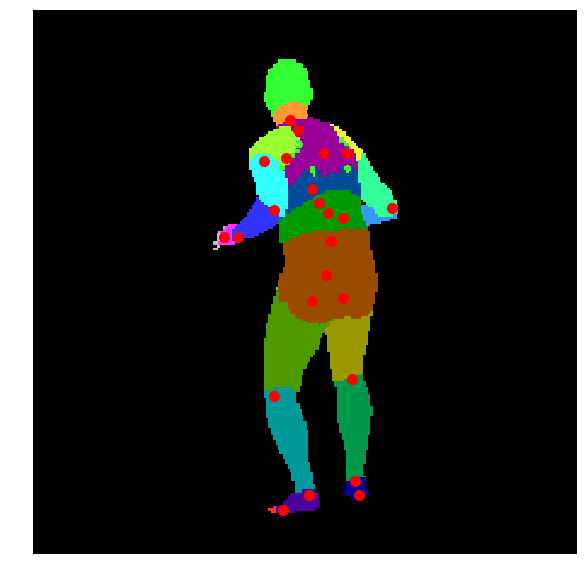
\includegraphics[scale=0.2]{surreal_joints.png}
\end{subfigure}
\begin{subfigure}{.45\textwidth}
  \centering
  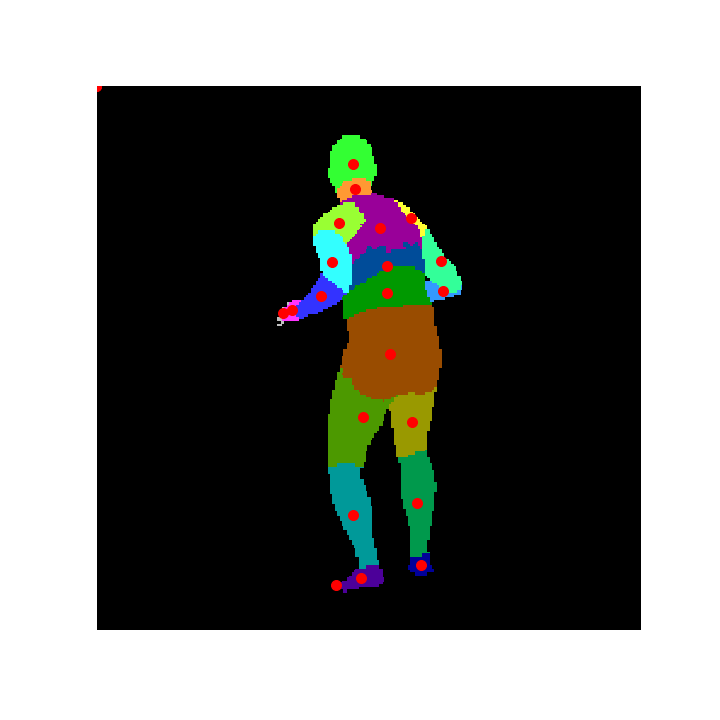
\includegraphics[scale=0.2]{central_point_parts.png}
\end{subfigure}
\caption{Location of the different joints. \textbf{Left}: joints provided by the SURREAL dataset. \textbf{Right}: central part point location.}
\label{hourglass:joints}
\end{figure}


The next experiment consists in the following: include another module (or modules) in parallel devoted to another task. As the original network was devoted to pose estimation (body joint location) the auxiliary task has been defined to be this original purpose. As seen in \ref{hourglass:multitask} the experiment consists in deviate the output of certain chosen module an introduce it both in the ordinary next module and into another parallel module. This new branch will be dedicated to joint location so ground truths must be generated or chosen. In this case, the SURREAL dataset provide (x,y) coordinates. Nevertheless, another option, if these information is not had is to consider the central point location of each of the body parts. Both joint types are shown in \ref{hourglass:joints}.\\

The purpose of this experiment is to see if adding this branch devoted to another task can help improve the results on the segmentation task. The junction between of both types of data is obvious since the joints indicate a delineation of the figure and also its position. However, the intention is not to obtain results on joint location but to see if this improves semantic segmentation.\\


\begin{figure}
\centering
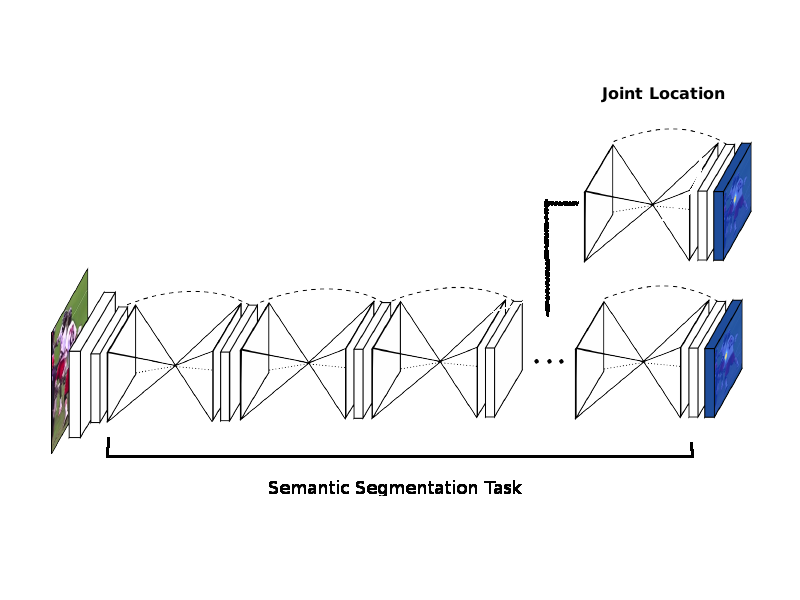
\includegraphics[scale=0.4]{multitask.png}
\caption{Representation of the multitask stacked hourglass. In this case with only one module devoted to the auxiliary task. The whole main network is devoted to semantic segmentation while the parallel module is devoted to joint location.}
\label{hourglass:multitask}
\end{figure}




\subsubsection{Results and analysis}

In this section performance results will be shown regarding the plain hourglass, the different resolutions experiment and the experiment of adding a joint detection branch.\\

In Figure \ref{hourglass:resultsplot}, the training loss and mIoU performance can be observed for three versions of the hourglass network: original, with different resolution ground truths and with a multi-task branch. As observed, the results are really poor in the case of the different resolution experiment. The fact that the hourglass network is thought to refine the same prediction through the consecutive modules seems to be the key fact in this failure. As in this case the prediction is different in each of the modules this refinement is not produced at its optimal behavior and performance is lost. In the case of the head the results in the validation set are several points below the original structure. This might be due to the different data type structure of the two related tasks: semantic segmentation of the body and joint localization. Joint position maybe misleads the position of each of the parts. Hence, and given the results,these two experiments as options of improving the original structure are dismissed.\\

\begin{figure}
\centering
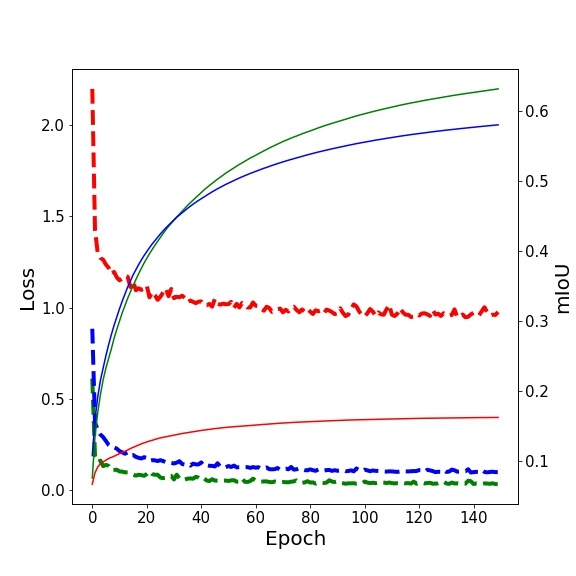
\includegraphics[scale=0.4]{loss_plot_GTnormal.jpg}
\caption{Plot of the loss and mIoU performance on the validation set while training. Dashed lines represent loss while solid lines represent mIoU values. Red lines correspond to the different resolutions scheme, blue lines to the scheme with the joint location branch and green lines to the original net.}
\label{hourglass:resultsplot}
\end{figure}

\begin{table}[h!]
  \begin{center}
    
    \begin{tabular}{|c|c|c|c|} % <-- Changed to S here.
      \textbf{Architecture} & \textbf{mIoU ($\%$)} & \textbf{Accuracy ($\%$)} & \textbf{F1 ($\%$)} \\
      \hline
      Original & 63.19 & 98.75 & 95.24\\
      \hline
      O. + GT resolutions & 16.22 & 90.58 & 61.98\\  
      \hline
      O. + Multitask Head & 58.05 & 97.18 & 96.05\\
    \end{tabular}
    \caption{Performance results on validation dataset for the original structure, the original structure plus different GT resolutions and the original structure plus a 2 module head devoted to joint estimation.}
    \label{hourglass:table1}
  \end{center}
\end{table}

Regarding results on the validation data set, the previously seen results can be ratified in Table \ref{hourglass:table1}: the original structure is way up both experiments. It has to be noted the poor results obtained with the resolutions frame. Regarding accuracy per class the same can be observed in Table \ref{hourglass:table2}. Here, it can be seen that although the original architecture obtains a better mIoU, the best results regarding accuracy per class are obtained by the multi task scheme. This may be due to the help provided by the joint localization. \\

\begin{table}[h!]
  \begin{center}
    \resizebox{\textwidth}{!}{
    \begin{tabular}{|c|c|c|c|c|c|c|c|c|c|c|c|c|c|c|c|c|c|c|c|c|c|c|} % <-- Changed to S here.
    &\textbf{mIoU ($\%$)}&\multicolumn{12}{c}{\textbf{Accuracy per Class}($\%$)}\\
    \hline
      \textbf{Architecture} & \textbf{All Classes} & \textbf{All classes}&\textbf{Background} & \textbf{Head} & \textbf{Torso} & \textbf{U.Legs}& \textbf{L.Legs} & \textbf{Neck} & \textbf{Shoulder} & \textbf{U.Arms}& \textbf{L.Arms}& \textbf{Feets}& \textbf{Hands}& \textbf{Fingers} & \textbf{Toes}  \\
      \hline
      Original & 63.19 & 98.75 & 99.82 & 37.81 & 32.63 & 37.58 & 37.59 & 30.46 & 22.75 & 24.29 & 18.87 & 33.87 & 9.86 & 5.97 & 14.52\\
 	  \hline
      O. + GT resolutions & 16.22 & 61.8 & 99.09 & 0.0 & 35.20 & 39.54 & 0.05 & 0.0 & 0.21 & 2.2 & 19.28 & 0.0 & 7.15 & 0.0 & 0.0\\  
      \hline
      O + Multitask Head & 58.05 & 96.05 & 99.76 & 93.38 & 79.38 & 85.76 &  86.0 & 59.72 & 59.16 & 
71.19 & 70.68 & 53.08 & 55.73 & 35.75 & 27.85 \\

    \end{tabular}}
    \caption{Performance results  of accuracy (overall and for each class) on the validation set for the original stacked hourglass structure, the original plus different ground truth (GT) resolutions and the original plus the multitask head. }
    \label{hourglass:table2}
  \end{center}
\end{table}

Finally, the best performing scheme has been, regarding mIoU, the original one. Hence, in Table \ref{hourglass:table3} results on the test set are shown. Note the good results obtained on it, although it does not even arrive to mark set by the original pape: 69.7$\%$. Nevertheless, qualitative results are quite precise, as can be shown in Figure \ref{hourglass:inference}. In some inference results, little body parts, such as fingers, are well shaped.\\

\begin{table}[h!]
  \begin{center}
    
    \begin{tabular}{|c|c|c|c|} % <-- Changed to S here.
      \textbf{Architecture} & \textbf{mIoU ($\%$)} & \textbf{Accuracy ($\%$)} & \textbf{F1 ($\%$)} \\
      \hline
      Original & 55.32 & 97.02 & 93.07\\
      \hline
    \end{tabular}
    \caption{Performance results on test dataset for the original structure.}
    \label{hourglass:table3}
  \end{center}
\end{table}

\begin{figure}
\centering
\begin{subfigure}{.19\textwidth}
\centering
  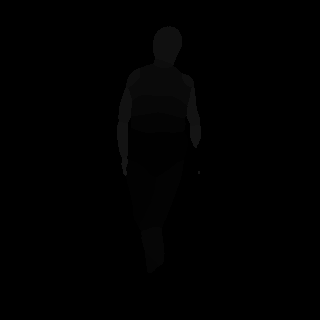
\includegraphics[scale=0.3]{ung_104_36_c0011_segm_7.png}
\end{subfigure}
\begin{subfigure}{.19\textwidth}
  \centering
  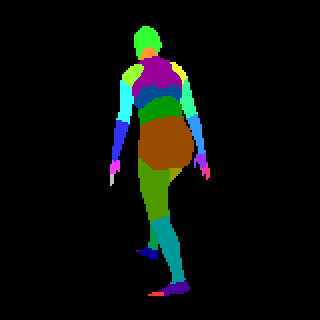
\includegraphics[scale=0.3]{36_10_c0019_segm_10.png}
\end{subfigure}
\begin{subfigure}{.19\textwidth}
  \centering
  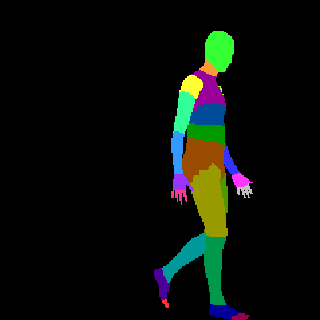
\includegraphics[scale=0.3]{40_02_c0011_segm_19.png}
\end{subfigure}
\begin{subfigure}{.19\textwidth}
  \centering
  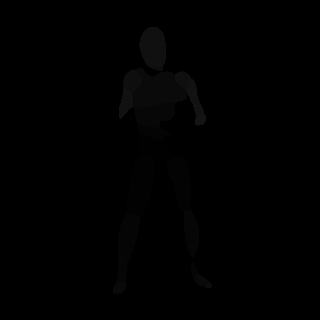
\includegraphics[scale=0.3]{104_52_c0002_segm_64.png}\\
\end{subfigure}\\
\begin{subfigure}{.198\textwidth}
\centering
  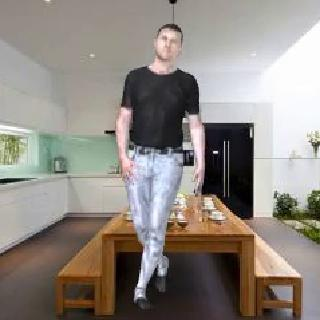
\includegraphics[scale=0.295]{ung_104_36_c0011_7.jpg}
\end{subfigure}%
\begin{subfigure}{.19\textwidth}
  \centering
  \includegraphics[scale=0.295]{36_10_c0019_10.jpg}
\end{subfigure}
\begin{subfigure}{.19\textwidth}
  \centering
  \includegraphics[scale=0.295]{40_02_c0011_19.jpg}
\end{subfigure}
\begin{subfigure}{.189\textwidth}
  \centering
  \includegraphics[scale=0.2945]{104_52_c0002_64.jpg}
\end{subfigure}

\caption{First row: ground truth examples. Second row: inference results with best Hourglass model.}
\label{hourglass:inference}
\end{figure}

 
% Chapter 2

\chapter{Network Comparison and Conclusions} % Main chapter title

\label{Chapter3} % For referencing the chapter elsewhere, use \ref{Chapter1} 

%----------------------------------------------------------------------------------------


%----------------------------------------------------------------------------------------

\section{Network Comparison}

Until now, three different networks has been studied but no comparison has been established between them. In this section qualitative and quantitative results from the best scheme of each network will be compared and possible reasons of the results will be elaborated.\\

\begin{table}[h!]
  \begin{center}
    
    \begin{tabular}{|c|c|c|c|} % <-- Changed to S here.
    \hline
      \textbf{} & \textbf{ ICNet} & \textbf{SegNet} & \textbf{Stacked Hourglass} \\
      \hline
      Number of trainable variables & 6.743.733 & 5.904.921 & 14.804.962\\     
      \hline
    \end{tabular}
    \caption{Number of trainable parameters for each of the networks (best performing version}
    \label{final:table3}
  \end{center}
\end{table}

In Table \ref{final:table1} results regarding the three main metrics (mIoU, F1 and Accuracy) in the test set are shown. As seen the best performing one is the stacked hourglass. There are two important comments to be made: one reason to this outstanding performance compared to the other two networks could be the fact that the network is defined for the human body. Nevertheless, as a second comment, it could be argued that in this study the number of parameters has not been equalized and then, as the stacked hourglass is bigger than the other two it is natural that it has a better performance. The same problem could be stated between ICNet and SegNet but only with regards the number of parameters. In Table \ref{final:table3} the number of parameters of each of the best performing networks can be checked. As seen the Stacked Hourglass has more than double parameters compared to ICNet.\\
 
\begin{table}[h!]
  \begin{center}
    
    \begin{tabular}{|c|c|c|c|} % <-- Changed to S here.
      \textbf{Architecture} & \textbf{mIoU ($\%$)} & \textbf{Accuracy ($\%$)} & \textbf{F1 ($\%$)} \\
      \hline
      ICNet & 45.14 & 95.76 & 89.73\\
      \hline
      SegNet & 33.59 & 94.62  & 44.32 \\  
      \hline
      Stacked Hourglass & 55.32 & 97.02 & 93.07\\
    \end{tabular}
    \caption{Performance results on test set for the best performing scheme of each of the three networks selected.}
    \label{final:table1}
  \end{center}
\end{table}

Regarding accuracy per class, results can be observed in Table \ref{final:table2}. As seen both ICNet and Segnet show similar results with poorer results in low pixel area classes. On the contrary, the Stacked Hourglass has a more balanced result with a certain and significant improvement in the classes with low number of pixels. Nevertheless, the same problem of size commented before can be associated to this results. Hence the good balancing of the class accuracy results of the Stacked Hourglass network could be due to its size/complexity or its affinity towards human body data.\\


\begin{table}[h!]
  \begin{center}
    \resizebox{\textwidth}{!}{
    \begin{tabular}{|c|c|c|c|c|c|c|c|c|c|c|c|c|c|c|c|c|c|c|c|c|c|c|} % <-- Changed to S here.
      \textbf{Architecture} & \textbf{All classes}&\textbf{Background} & \textbf{Head} & \textbf{Torso} & \textbf{U.Legs}& \textbf{L.Legs} & \textbf{Neck} & \textbf{Shoulder} & \textbf{U.Arms}& \textbf{L.Arms}& \textbf{Feets}& \textbf{Hands}& \textbf{Fingers} & \textbf{Toes}  \\
      ICNet & 95.7 & 89.3 & 60.6 & 76.7 & 78.5 & 64.9 & 65.9 &10.6 & 41.9 & 64.5 & 59.8 & 43.1 & 33.9 & 42.5 \\
      \hline
      SegNet & 94.3 & 99.8 & 68.6 & 63.3 & 56.7 & 45.0 & 30.4 & 32.3 & 41.7 & 23.5 & 22.8 & 10.9 & 6.0 & 4.7\\
      \hline
      Stacked Hourglass  & 98.4 & 99.7 & 74.5 & 76.4 & 79.9 & 78.2 & 64.8 & 44.7 & 49.4 & 52.2 & 48.6 & 41.0 & 45.3 & 55.4\\
 	      \end{tabular}}
    \caption{Performance results on test dataset regarding accuracy per class for the best performing schemes of each of the three structures}
    \label{final:table2}
  \end{center}
\end{table}


In Figure \ref{final:inference} qualitative results of the best performing schemes of each network can be observed. As seen the best quality is shown by Stacked Hourglass. This could be due to the continuous refinement of the output in the pipeline. The poorest results are shown by SegNet Basic. This could be due to the low number of parameters or to the network configuration. Since it has only one top-down bottom-up process refinement is not carried out. Also, in the upsampling process information is lost, although skip connections help to avoid this loss. Nevertheless, since only indexes, and not full maps are stored, the recovering is not complete (although it speeds up the process). Regarding ICNet the results are pretty good but not as good as in Stacked Hourglass. This could be done to the use of the full resolution branch only when doing inference. This causes loss of precision but enhances inference speed.\\



\begin{figure}
\centering
\begin{subfigure}{.19\textwidth}
\centering
  \includegraphics[scale=0.3]{ung_104_36_c0011_segm_7.png}
\end{subfigure}
\begin{subfigure}{.19\textwidth}
  \centering
  \includegraphics[scale=0.3]{36_10_c0019_segm_10.png}
\end{subfigure}
\begin{subfigure}{.19\textwidth}
  \centering
  \includegraphics[scale=0.3]{40_02_c0011_segm_19.png}
\end{subfigure}
\begin{subfigure}{.19\textwidth}
  \centering
  \includegraphics[scale=0.3]{104_52_c0002_segm_64.png}\\
\end{subfigure}\\
\begin{subfigure}{.198\textwidth}
\centering
  \includegraphics[scale=0.295]{ung_104_36_c0011_7_ice.jpg}
\end{subfigure}%
\begin{subfigure}{.19\textwidth}
  \centering
  \includegraphics[scale=0.295]{36_10_c0019_10_ice.jpg}
\end{subfigure}
\begin{subfigure}{.19\textwidth}
  \centering
  \includegraphics[scale=0.295]{40_02_c0011_19_ice.jpg}
\end{subfigure}
\begin{subfigure}{.189\textwidth}
  \centering
  \includegraphics[scale=0.296]{104_52_c0002_64_ice.jpg}
\end{subfigure}\\
\begin{subfigure}{.19\textwidth}
\centering
  \includegraphics[scale=0.3]{ung_104_36_c0011_segm_7_seg.png}
\end{subfigure}
\begin{subfigure}{.19\textwidth}
  \centering
  \includegraphics[scale=0.3]{36_10_c0019_segm_10_seg.png}
\end{subfigure}
\begin{subfigure}{.19\textwidth}
  \centering
  \includegraphics[scale=0.3]{40_02_c0011_segm_19_seg.png}
\end{subfigure}
\begin{subfigure}{.19\textwidth}
  \centering
  \includegraphics[scale=0.3]{104_52_c0002_segm_64_seg.png}\\
\end{subfigure}\\
\begin{subfigure}{.198\textwidth}
\centering
  \includegraphics[scale=0.295]{ung_104_36_c0011_7.jpg}
\end{subfigure}%
\begin{subfigure}{.19\textwidth}
  \centering
  \includegraphics[scale=0.295]{36_10_c0019_10.jpg}
\end{subfigure}
\begin{subfigure}{.19\textwidth}
  \centering
  \includegraphics[scale=0.295]{40_02_c0011_19.jpg}
\end{subfigure}
\begin{subfigure}{.189\textwidth}
  \centering
  \includegraphics[scale=0.296]{104_52_c0002_64.jpg}
\end{subfigure}

\caption{First row: ground truth examples.  Second row: inference results with best ICNet model. Third row: inference results with best Segnet model. Fourth row: inference results with best Hourglass model.}
\label{final:inference}
\end{figure}

 



\section{Conclusions}
 	   
In this study we have analyzed three different structures which have as a main component convolution layers. ICNet focuses on different resolution samples of the same image through different branches to speed up inference but maintaining accuracy. SegNet, in our case SegNet Basic, uses an encoder decoder network with skip connections to avoid on-memory overloading and fast inference. And finally, Stacked Hourglass, which through its use of consecutive modules and residual components enables the refining process of the output produced. \\

In two different configurations of experiments, one for generally purposed networks and another for specific purposed networks, we have tried to improve the results obtained with these networks with regards the chosen dataset: SURREAL. Unfortunately, in almost none of them the results has been positive. In the first set of networks, the only positive results has been the doubling of filters in Segnet but not any other network configuration. In the second part, none of the new configurations have improved the results.\\

As a main drawback of this study it can be emphasized the fact that the networks were not in size/complexity equality: they differed in the number of parameters. Hence, this includes a bias to the study. Nevertheless, this  has not prevented us to satisfactorily obtain results from the three and be able to establish the differences in performance and use.\\

Regarding the future work that could be done, there are two main points: one is to include more networks to the study to make it more diverse and representative, and the second is to include the previously named problem, that is, configure the networks so, more or less, all have the same size or are similar in terms of complexity.\\

As a conclusion, this study has been centered on the examination and performance of three different fully convolutional networks applied to the SURREAL dataset. As a matter of fact, the Stacked Hourglass network has proven to be far better than the other two networks, although it has not been possible to establish clearly the reason: being size, structure definition or data type affinity. The results on the modifications of the networks have not been positive but have enabled the student to acquire a certain level, regarding both programming skills and field concepts, to carry on further and deeper studies. \\
%\include{Chapters/Chapter4} 
%\include{Chapters/Chapter5} 

%----------------------------------------------------------------------------------------
%	THESIS CONTENT - APPENDICES
%----------------------------------------------------------------------------------------

\appendix % Cue to tell LaTeX that the following "chapters" are Appendices

% Include the appendices of the thesis as separate files from the Appendices folder
% Uncomment the lines as you write the Appendices

%% Appendix A

\chapter{Frequently Asked Questions} % Main appendix title

\label{AppendixA} % For referencing this appendix elsewhere, use \ref{AppendixA}

\section{How do I change the colors of links?}

The color of links can be changed to your liking using:

{\small\verb!\hypersetup{urlcolor=red}!}, or

{\small\verb!\hypersetup{citecolor=green}!}, or

{\small\verb!\hypersetup{allcolor=blue}!}.

\noindent If you want to completely hide the links, you can use:

{\small\verb!\hypersetup{allcolors=.}!}, or even better: 

{\small\verb!\hypersetup{hidelinks}!}.

\noindent If you want to have obvious links in the PDF but not the printed text, use:

{\small\verb!\hypersetup{colorlinks=false}!}.

%\include{Appendices/AppendixB}
%\include{Appendices/AppendixC}

%----------------------------------------------------------------------------------------
%	BIBLIOGRAPHY
%----------------------------------------------------------------------------------------

\printbibliography[heading=bibintoc]

%----------------------------------------------------------------------------------------

\end{document}  
